


\documentclass[journal]{IEEEtran}
%\documentclass[runningheads]{llncs}
% added by kahraman


\usepackage{xr-hyper} 
\usepackage{hyperref} 




\usepackage[acronym,nonumberlist,nogroupskip,style=super]{glossaries}
\usepackage{hyperref}
\newacronym{iot}{IoT}{Internet of Things} %\gls{label}


%added from previous article begin

\usepackage{cite}
\usepackage{amsmath,amssymb,amsfonts}
%\usepackage{algorithmic}
\usepackage{graphicx}
\usepackage{textcomp}
\usepackage{bmpsize}
\usepackage[dvipsnames]{xcolor}
\usepackage{lipsum}

%\usepackage[hyphens]{url} %kahraman added
%\usepackage[colorlinks=true,urlcolor=black]{hyperref}


%\usepackage[labelfont=bf]{caption}
\usepackage[font=footnotesize,labelfont=bf]{caption}

%\captionsetup[table]{skip=10pt}
\newcommand{\cmark}{\ding{51}}%
\newcommand{\xmark}{\ding{55}}%

\usepackage[export]{adjustbox}
%\usepackage{subcaption}	 
\usepackage{pifont}
\usepackage{multirow}
\usepackage{tabularx}
%\usepackage{algpseudocode} 
\usepackage{algorithmicx}
\usepackage[noend]{algpseudocode}
\usepackage[T1]{fontenc}
\usepackage{algorithm} 
\usepackage{subfig}	
\usepackage{soul}
\usepackage{booktabs}

\usepackage{multirow}
\usepackage{rotating}
\usepackage{booktabs}


\usepackage{siunitx,etoolbox}

%\usepackage[table]{xcolor}
\usepackage{color, colortbl}

\usepackage{comment}
\usepackage{lscape}
\usepackage{fontawesome5}
%added from previous article end

% correct bad hyphenation here
%\hyphenation{op-tical net-works semi-conduc-tor}


\begin{document}
%
% paper title
% Titles are generally capitalized except for words such as a, an, and, as,
% at, but, by, for, in, nor, of, on, or, the, to and up, which are usually
% not capitalized unless they are the first or last word of the title.
% Linebreaks \\ can be used within to get better formatting as desired.
% Do not put math or special symbols in the title.
\title{Applying IoTDevID to a New Dataset: the CIC-IoT-2022 Case Study}
%\title{IoTDevID: Behavior-Based IoT Device Identification}

\author{Kahraman~Kostas,
	Mike~Just,
	and~Michael~A.~Lones% <-this % stops a space
\thanks{K.~Kostas, M.~Just,	and~M.~A.~Lones  are with the Department of Computer Science, Heriot-Watt University, Edinburgh EH14 4AS, UK,  e-mail: kk97, m.just, m.lones@hw.ac.uk}
\thanks{Kahraman Kostas supported by Republic of Turkey - Ministry of National Education}}% <-this % stops a space

% note the % following the last \IEEEmembership and also \thanks - 
% these prevent an unwanted space from occurring between the last author name
% and the end of the author line. i.e., if you had this:
% 
% \author{....lastname \thanks{...} \thanks{...} }
%                     ^------------^------------^----Do not want these spaces!
%
% a space would be appended to the last name and could cause every name on that
% line to be shifted left slightly. This is one of those "LaTeX things". For
% instance, "\textbf{A} \textbf{B}" will typeset as "A B" not "AB". To get
% "AB" then you have to do: "\textbf{A}\textbf{B}"
% \thanks is no different in this regard, so shield the last } of each \thanks
% that ends a line with a % and do not let a space in before the next \thanks.
% Spaces after \IEEEmembership other than the last one are OK (and needed) as
% you are supposed to have spaces between the names. For what it is worth,
% this is a minor point as most people would not even notice if the said evil
% space somehow managed to creep in.



% The paper headers
%%%%%%%%%%%%%%%%%%%\markboth{Journal of \LaTeX\ Class Files,~Vol.~14, No.~8, August~2015}%
%%%%%%%%%%%%%%%%%%%{Shell \MakeLowercase{\textit{et al.}}: Bare Demo of IEEEtran.cls for IEEE Journals}
% The only time the second header will appear is for the odd numbered pages
% after the title page when using the twoside option.
% 
% *** Note that you probably will NOT want to include the author's ***
% *** name in the headers of peer review papers.                   ***
% You can use \ifCLASSOPTIONpeerreview for conditional compilation here if
% you desire.



% If you want to put a publisher's ID mark on the page you can do it like
% this:
%\IEEEpubid{0000--0000/00\$00.00~\copyright~2015 IEEE}
% Remember, if you use this you must call \IEEEpubidadjcol in the second
% column for its text to clear the IEEEpubid mark.



% use for special paper notices
%\IEEEspecialpapernotice{(Invited Paper)}




% make the title area
\maketitle

% As a general rule, do not put math, special symbols or citations
% in the abstract or keywords.
\begin{abstract}
In this paper, we have examined under various headings the aspects to be considered in device identification studies using machine learning methods, common mistakes that may occur and how to avoid them. Our paper briefly touched upon the following topics: identification methods and their pros and cons, available data types and properties, common mistakes made during feature extraction and their solutions, what to consider about the use of machine learning methods, and how to choose appropriate evaluation methods.
\end{abstract}

% Note that keywords are not normally used for peerreview papers.
\begin{IEEEkeywords}
IoT security, IoT fingerprinting, machine learning, device identification
\end{IEEEkeywords}



\section{Introduction}


Especially in the last two decades, we have heard the concept of the Internet of Things a lot. IoT can be defined as any kind of physical device with processing capability that can be connected to the internet or other devices~\cite{IoT2023What}.  IoT, which acts as a link between the digital world and the real world, are becoming increasingly present in our lives every day. Not only in our digital life on the computer/phone but also as a part of our home, work or street, they permeate every point of our physical lives. Today, the number of IoT has exceeded 10 billion, which is expected to reach 27 billion by 2025\cite{IoT2023sta}. 

This rapid progress brings along many problems.  In a rapidly growing market, a variety of devices have been developed by many companies for many purposes in a short time. Due to the nature of IoT devices, these devices have very different hardware and software characteristics.  For example, a smart kettle and a smart door lock are vastly different from each other, even though they are both IoT. The heterogeneity of these devices, combined with vulnerabilities from manufacturers and the often unfamiliar interfaces of the devices, make them potentially dangerous. According to statistics, an IoT device connected to the internet is attacked within 5 minutes and becomes the target of a specialised attack within 24 hours~\cite{modi_2019}. 


In order to cope with these attacks, it is essential to keep the devices up to date, identify the vulnerabilities they carry and find solutions for them. These devices may need to be updated, restricted or isolated from other devices depending on the vulnerabilities they carry. In any measure to be taken, the first step will be to identify the device. Necessary measures can be taken for the identified device by scanning for vulnerabilities from a source such as the CVE~\cite{cve} database.  However, the heterogeneous structure of IoT devices makes the device identification process very difficult. In this regard, many researchers are applying machine learning-based identification for more efficient solutions. 

We created IoTDevID~\cite{kostas2022IoTDevID} to address the device identification problem. IoTDevID works at the individual packet level to identify IoT devices, whether IP or non-IP (such as ZWave, ZigBee, or Bluetooth). In doing so, it provides a high detection rate thanks to its incorporated aggregation algorithm, overcoming the disadvantage of low performance of using individual packets.


IoTDevID uses only publicly available data and its scripts is also publicly available~\footnote{Materials available at: github.com/kahramankostas/IoTDevID-CIC.}. It is therefore a transparent, reliable and repeatable study.

In the multi-layer feature selection process, device and session-based identifying features that cause over fitting are discarded, and the most appropriate feature set is created by using the genetic algorithm. In this context, IoTDevID provides generalisable and robust models.  In this study, we will validate our previously created IoTDevID by applying it to a new dataset, the CIC-IoT-22 dataset. In this way, we will test the robustness and generalisability of our method with another dataset.


\section{Related Work}

In this section, we will review some studies in the literature on device identification using machine learning. Device identification aims to classify devices by using feature sets (fingerprints) obtained from network data as input.  These features are usually derived from individual packet headers or payload, but some studies have also used flow features. There are three different approaches to the classification process~\cite{yadav2020position}:
\textbf{Unique Identification:} By accepting each of the devices as unique, a separate class is created for each device~\cite{hamad2019iot}.\\
\textbf{Type Identification:}  Identification is performed according to the device type. If there are multiple devices of the same brand and model, they are seen as a single class~\cite{miettinen2017iot}.\\
\textbf{Class Identification:}  Different devices that are not the same but have similar features, are gathered under a single class such as camera, speaker, or smart lamp~\cite{CIC}. Fig.~\ref{fig:3aproach} shows the labelling of CIC-IoT-22 dataset with three viewpoints. In the example containing 20 devices in total, 20 different labels are formed in the unique method, 13 different labels in the type method, and 3 different labels (Smart Lamp/Bulb, Speakers, and Smart Plug respectively) in the class method. 

\begin{figure}[ht]
	%	\vspace*{-3mm}
	\centerline{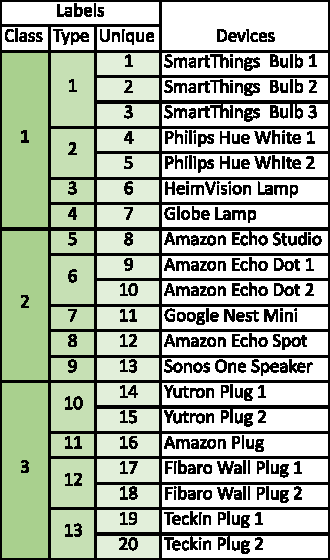
\includegraphics[width=0.61\columnwidth]{images/class.pdf}}
	\caption{The change of device labels of the CIC dataset according to 3 identification methods. In the unique method, each device is considered unique and labelled with this name, regardless of other devices. In the Type method, devices with the same brand and model are considered as a single device and share the same label. In the Type method, three devices that were originally labelled separately as SmartThings Bulb 1-2-3 are collected under the SmartThings Bulb label. In the Class method, devices with the same function are grouped under a single tag. For example, in the class column, 1,2,3 represent the categories Smart Lamp/Bulb, speaker, and smart plug respectively..}
	\label{fig:3aproach}
\end{figure}

In parallel to these three approaches, we can analyse the literature as follows. In order to perform a unique classification, a dataset must have more than one device of the same make and model. Hamad et al.\@~\cite{hamad2019iot} used the Aalto dataset which is suitable for this task in their work aiming at a unique classification. However, the unique classification cannot be achieved by using the individual packet features.   Therefore, this study used 67 features consisting of network statistics derived from 20-21 consecutive individual packet features. However, these are specific to the network in which they are produced.  If the same device or model is moved to another network, these network statistics will change and the model will no longer function. In this respect, flow-based features are more likely to be used in anomaly detection rather than device identification. Conversely, the use of individual packets is also inadequate for anomaly detection\cite{kostas2023AD}.


There are more studies using the Type classification. Among these, IoTSentinel~\cite{miettinen2017iot}, a pioneering study, is particularly noteworthy. In this study using Aalto data, 23 individual features extracted from packet headers are used. These features, which are taken from 12 packets without repetition, are combined under MAC address guidance to create a larger fingerprint.  This larger fingerprint is used as machine learning input.  This study uses the RF method to classify 17 out of 27 devices with an accuracy of over 95\% and, for 10 devices, the accuracy remains around 50\%. However, the work is very strictly dependent on the MAC address. Therefore, it cannot solve the transfer problem, where a MAC address represents more than one device.


Another work that uses the Aalto dataset is~\cite{aksoy2019automated}. In this study, using a genetic algorithm, 33 of the 212 features obtained from the packet headers were selected and 95\% accuracy was obtained using these features.  This study can be criticised for using overly specific features  (such as port numbers, TCP sequence, TCP
acknowledgment,  and IP ID) that may leak information about inter-packet interactions, and for using a partial dataset (23 out of 27 devices were used).

Another interesting work is IoTSense~\cite{bezawada2018behavioral}. This work creates a new feature set by improving IoTsentinel features. In this feature set, a 20-element feature set is created by adding 17 features from IoTsentinel and 3 yuk-based features. By combining 5 of these subsets, larger feature sets are obtained to feed the ML. Although no details are given in the study, we guess that MAC address is used to combine these 5 subsets. Although this study shows an accuracy of 99\%, the fact that the dataset used is not shared and that 4 out of 14 devices were discarded during the experiment makes the result unreliable. In addition, if the MAC address is used, it will suffer from the transfer problem.

The work done by Sivanathan  et al.\@\cite{sivanathan2018classifying} is very important in terms of providing another device identification dataset to the literature. Using NB and RF methods, the UNSW dataset containing 28 devices could be classified with 99\% accuracy. However, it can be criticised that in this study identifying features were used such as flow-based features, cipher suite, DNS queries, and  port numbers. In addition, some devices in the dataset were not included in the evaluation step.
Finally, we will evaluate the study by Dadkhah et al.\@\cite{CIC}. In this study, which introduced a new CIC-IoT-22 dataset to the literature, a class-based classification was used. The devices in the dataset are classified using 3 categories: Audio,
Camera, and
Home Automation. 12 machine learning methods were used in this study and 98\% accuracy was achieved. It is also interesting to note that during the testing phase, data from a different lab and different devices were used. Even though we used the data from this study, our results are not comparable, since we used type-based evaluation and they used class-based evaluation.  More information about the dataset used is given in the data section.




\begin{figure}[ht]
	%	\vspace*{-3mm}
	\centerline{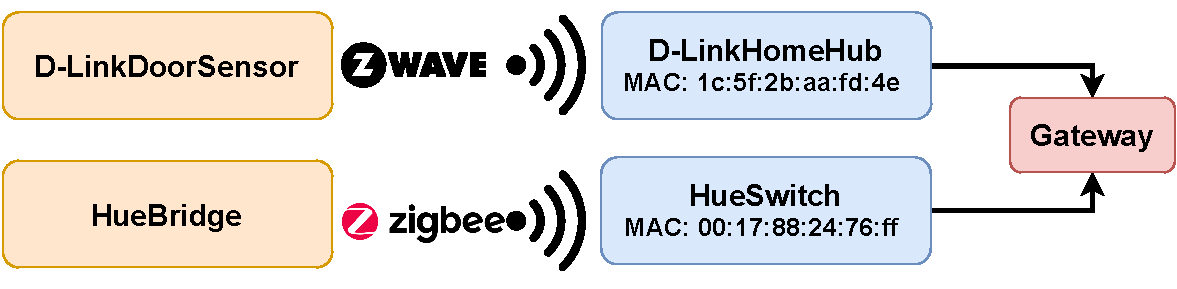
\includegraphics[width=1\columnwidth]{images/TraP.pdf}}
	\caption{Visualisation of the transfer problem in the Aalto dataset. The network data is collected at the gateway.  Between the HueBridge HueSwitch there is only Zigbee as a communication medium, between the HueSwitch  and gateway there is only Ethernet. Data from the HueBridge is decapsulated at the HueSwitch and re-encapsulated for transmission to the gateway. As a result of this process, both the HueBridge and HueSwitch share the same MAC address as the data is encapsulated on the same device (the same happens between D-LinkDoorSensor, D-LinkHomeHub and gateway). Therefore, studies that use MAC addresses to concatenate packets cannot overcome this problem.}
	\label{fig:transfer}
\end{figure}

To briefly summarise the "IoTDevID" work, we used the Aalto dataset for method development, analysis and feature extraction, and the UNSW dataset to demonstrate that the method is robust and generalisable. For features, we used features extracted from individual packages. After an extensive evaluation of machine learning methods, we decided on DT, which is quite acceptable in terms of performance, and also quite fast, making it very suitable for real life applications. We applied a multi-stage feature selection process, in the first step we discarded descriptive features, then we eliminated unimportant features by voting based on 6 different feature scores, and finally we generated the ideal feature set using a genetic algorithm. We achieved significant improvements in our results by using the aggregation algorithm. Compared to previous studies, we find that IoTDevID is significantly more successful. In this study, we will validate the work by applying IoTDevID to the CIC dataset.




\begin{figure}[ht]
	%	\vspace*{-3mm}
	\centerline{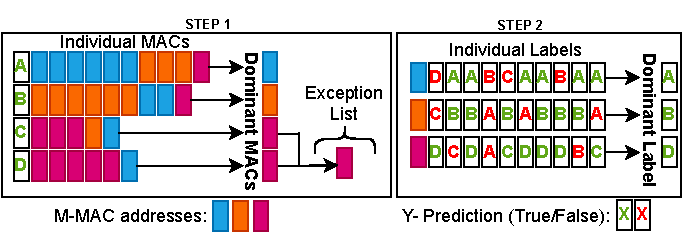
\includegraphics[width=1\columnwidth]{images/agregation.pdf}}
	\caption{The number of packets produced by the devices in the Aalto dataset.}
	\label{fig:pie}
\end{figure}






\section{MATERIALS AND METHODS}


dataset

One of the biggest problems in device identification studies is the lack of adequate datasets. The simulations used in many networking studies cannot be used in device identification studies, and the fact that the dataset can only be created with real device data is the most prominent of the difficulties. To create a proper device identification dataset, many types of IoT devices are needed, and the supply of these devices is a serious financial burden. In addition, normal data collection requires a long time, labour, and specialised space. In our baseline study, IoTDevID~\cite{Kostas2022IoTDevID}, we used two datasets, the Altoo  University~\cite{miettinen2017iot,aalto2017dataset} and UNSW datasets~\cite{sivanathan2018classifying}, which were produced for device identification studies. In this study, we used the Altoo dataset to develop our method and the second dataset to validate our results. In 2022, a new device identification dataset, CIC-IoT-22~\cite{CIC}, was made public.This dataset is very interesting as it contains many types and numbers of devices, contains the state of the devices under different conditions, and contains attack data in addition to benign data.  This dataset is very useful to demonstrate the usefulness, robustness, and generalisability of our method. 




In this dataset, data was collected in 6 different situations. These situations can be summarised as follows. 
In the \textbf{Power} state, each device is isolated from other devices and rebooted and the network packets related to this device are collected.
In the \textbf{Interactions} state, the device is interacted with by buttons, applications or voice commands and the network packets generated during this process are collected.
In \textbf{Scenarios}, the network data of these devices are collected in situations such as entering the house, leaving the house, unauthorised entry to the house at night and day or user error. 
In case of \textbf{attack} state, data is collected by applying Flood attacks and RTSP Brute Force attacks to the devices.
the \textbf{Idle} state consists of recording every 8-hour period for 30 days in the evening hours when the devices are working but not actively used.
The \textbf{active} state contains the data of the devices being used during the day for 30 days. This data is generated by people entering the lab and using the devices.

Some important points about the dataset:
In this study, the most important sections for us are IDLE and Active. In these two sections, enough data has been collected from almost all devices. Although it is stated on the paper that 60 devices were used in this process, according to our own experiments and the information provided in the dataset, these sections contain 40 devices. These 40 devices consist only of lan WIFI devices, they do not include Zigbee and z-wave devices. Zigbee and Z-Wave devices have data isolated from other devices, including power interaction and hede hodo, but these data are both very limited and do not contain normal usage data.








FE

Python, Scapy and WireShark were used for feature extraction. Only individual package-based features are used for feature extraction. Many of these features are derived from packet headers, but there are also payload-based features such as payload entropy and payload bytes. Although the feature exruction system created about 100 features in total (features and their descriptions can be found in Table~\ref{tab:features1}.), very few of these features, only the sub-features selected during the feature selection phase of the IoTDevID study, were used in the experiment.


Labelling:
Labelling was performed using the list of device names/MAC addresses couples in the dataset. In each fingerprint extracted, the source MAC address part was replaced with the given name and the MAC addresses not given in this list (5 MAC addresses that we believe belong to the hub, switch or the computer where the data is collected) were ignored.



Each of the pcap files we use for feature extraction contains network traffic recorded on a day, and is named with the date it was recorded.   For example, data recorded on 24.11.2021 is labelled A211124 if Active and I211124 if Idle. In this context, 30 IDLE and 24 active sessions were recorded. as a preliminary study,, we aimed to test the performance of all these sessions by comparing them with each other. In order to compare the sessions with each other, they should contain similar devices. Unfortunately, data was not collected from every device in every session, and in some sessions some devices did not generate any data at all. Table~\ref{tab:packets}.) shows how much data was generated by each device in each session in terms of network packets. Therefore, we only compare sessions that contain the same devices with each other. For this comparison, we create a session ID. In this ID, each device is represented by a binary digit. If the session has that device, it is indicated with 1, if not, it is indicated with 0. For example, if sessin1 contains devices A, and C but not device B, then the ID number is 101(ABC). Sessin1 can be compared to other sessions with the same ID number without any problem. In this context, we have created a 40-digit ID for each session according to totalling 40 devices.



The results we obtained by using devices with the same ID as training and test data are given in Fig.~\ref{fig:stepsofID}.  We used the F1 score to present these results for roughly two reasons. Firstly, unlike accuracy, f1 score gives reliable results on unbalanced data sets. Secondly, the F1 score does not only give overall results, but also allows us to analyse the results by class. When the results are analysed in this context, it is seen that the F1 score varies between 40\%-88\% in pairwise session comparisons. Another point we would like to draw attention to here is that this process is a multiple classification process with approximately 40\% classes. In this context, even 40 F1 is a much better result than chance/random success.


When the figures are analysed, it is seen that the results coinciding with specific dates in Fig.~\ref{fig:comp_1} (211108, 211109, 211206, 211208, 211223, 211225, 211228) are unsuccessful, on the other hand, when Fig.~\ref{fig:comp_2} is analysed, it is seen that the results in certain consecutive date ranges are more successful.




\begin{figure}[ht]
	%	\vspace*{-3mm}
	
	%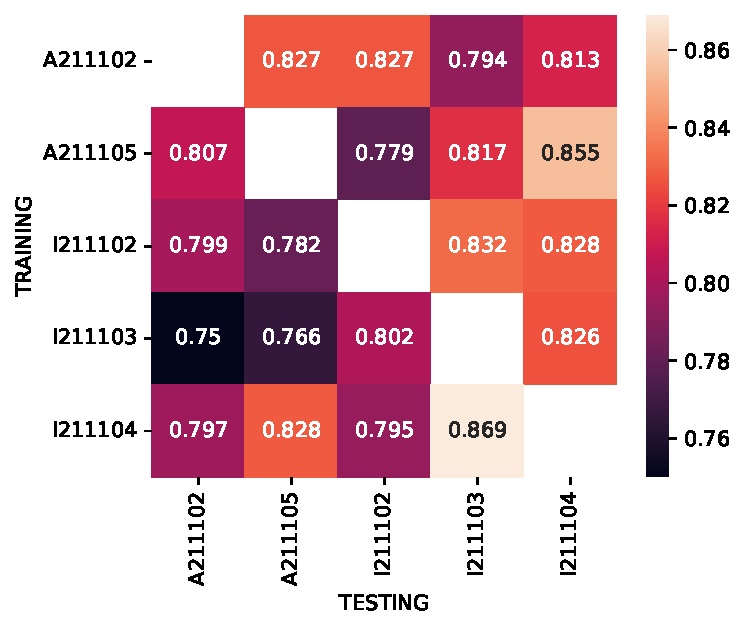
\includegraphics[width=0.6\columnwidth]{images/cm1.pdf}		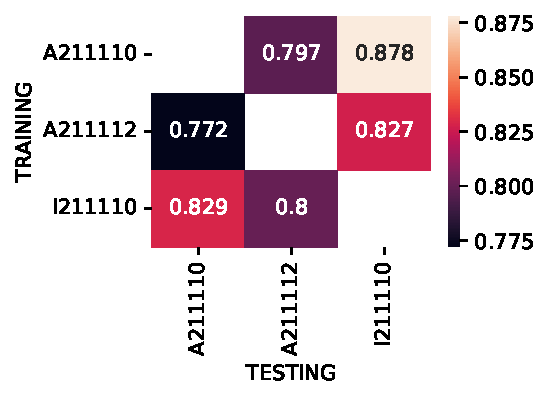
\includegraphics[width=0.5\columnwidth]{images/cm3.pdf}
	\subfloat[\label{fig:comp_1}\centering ]{{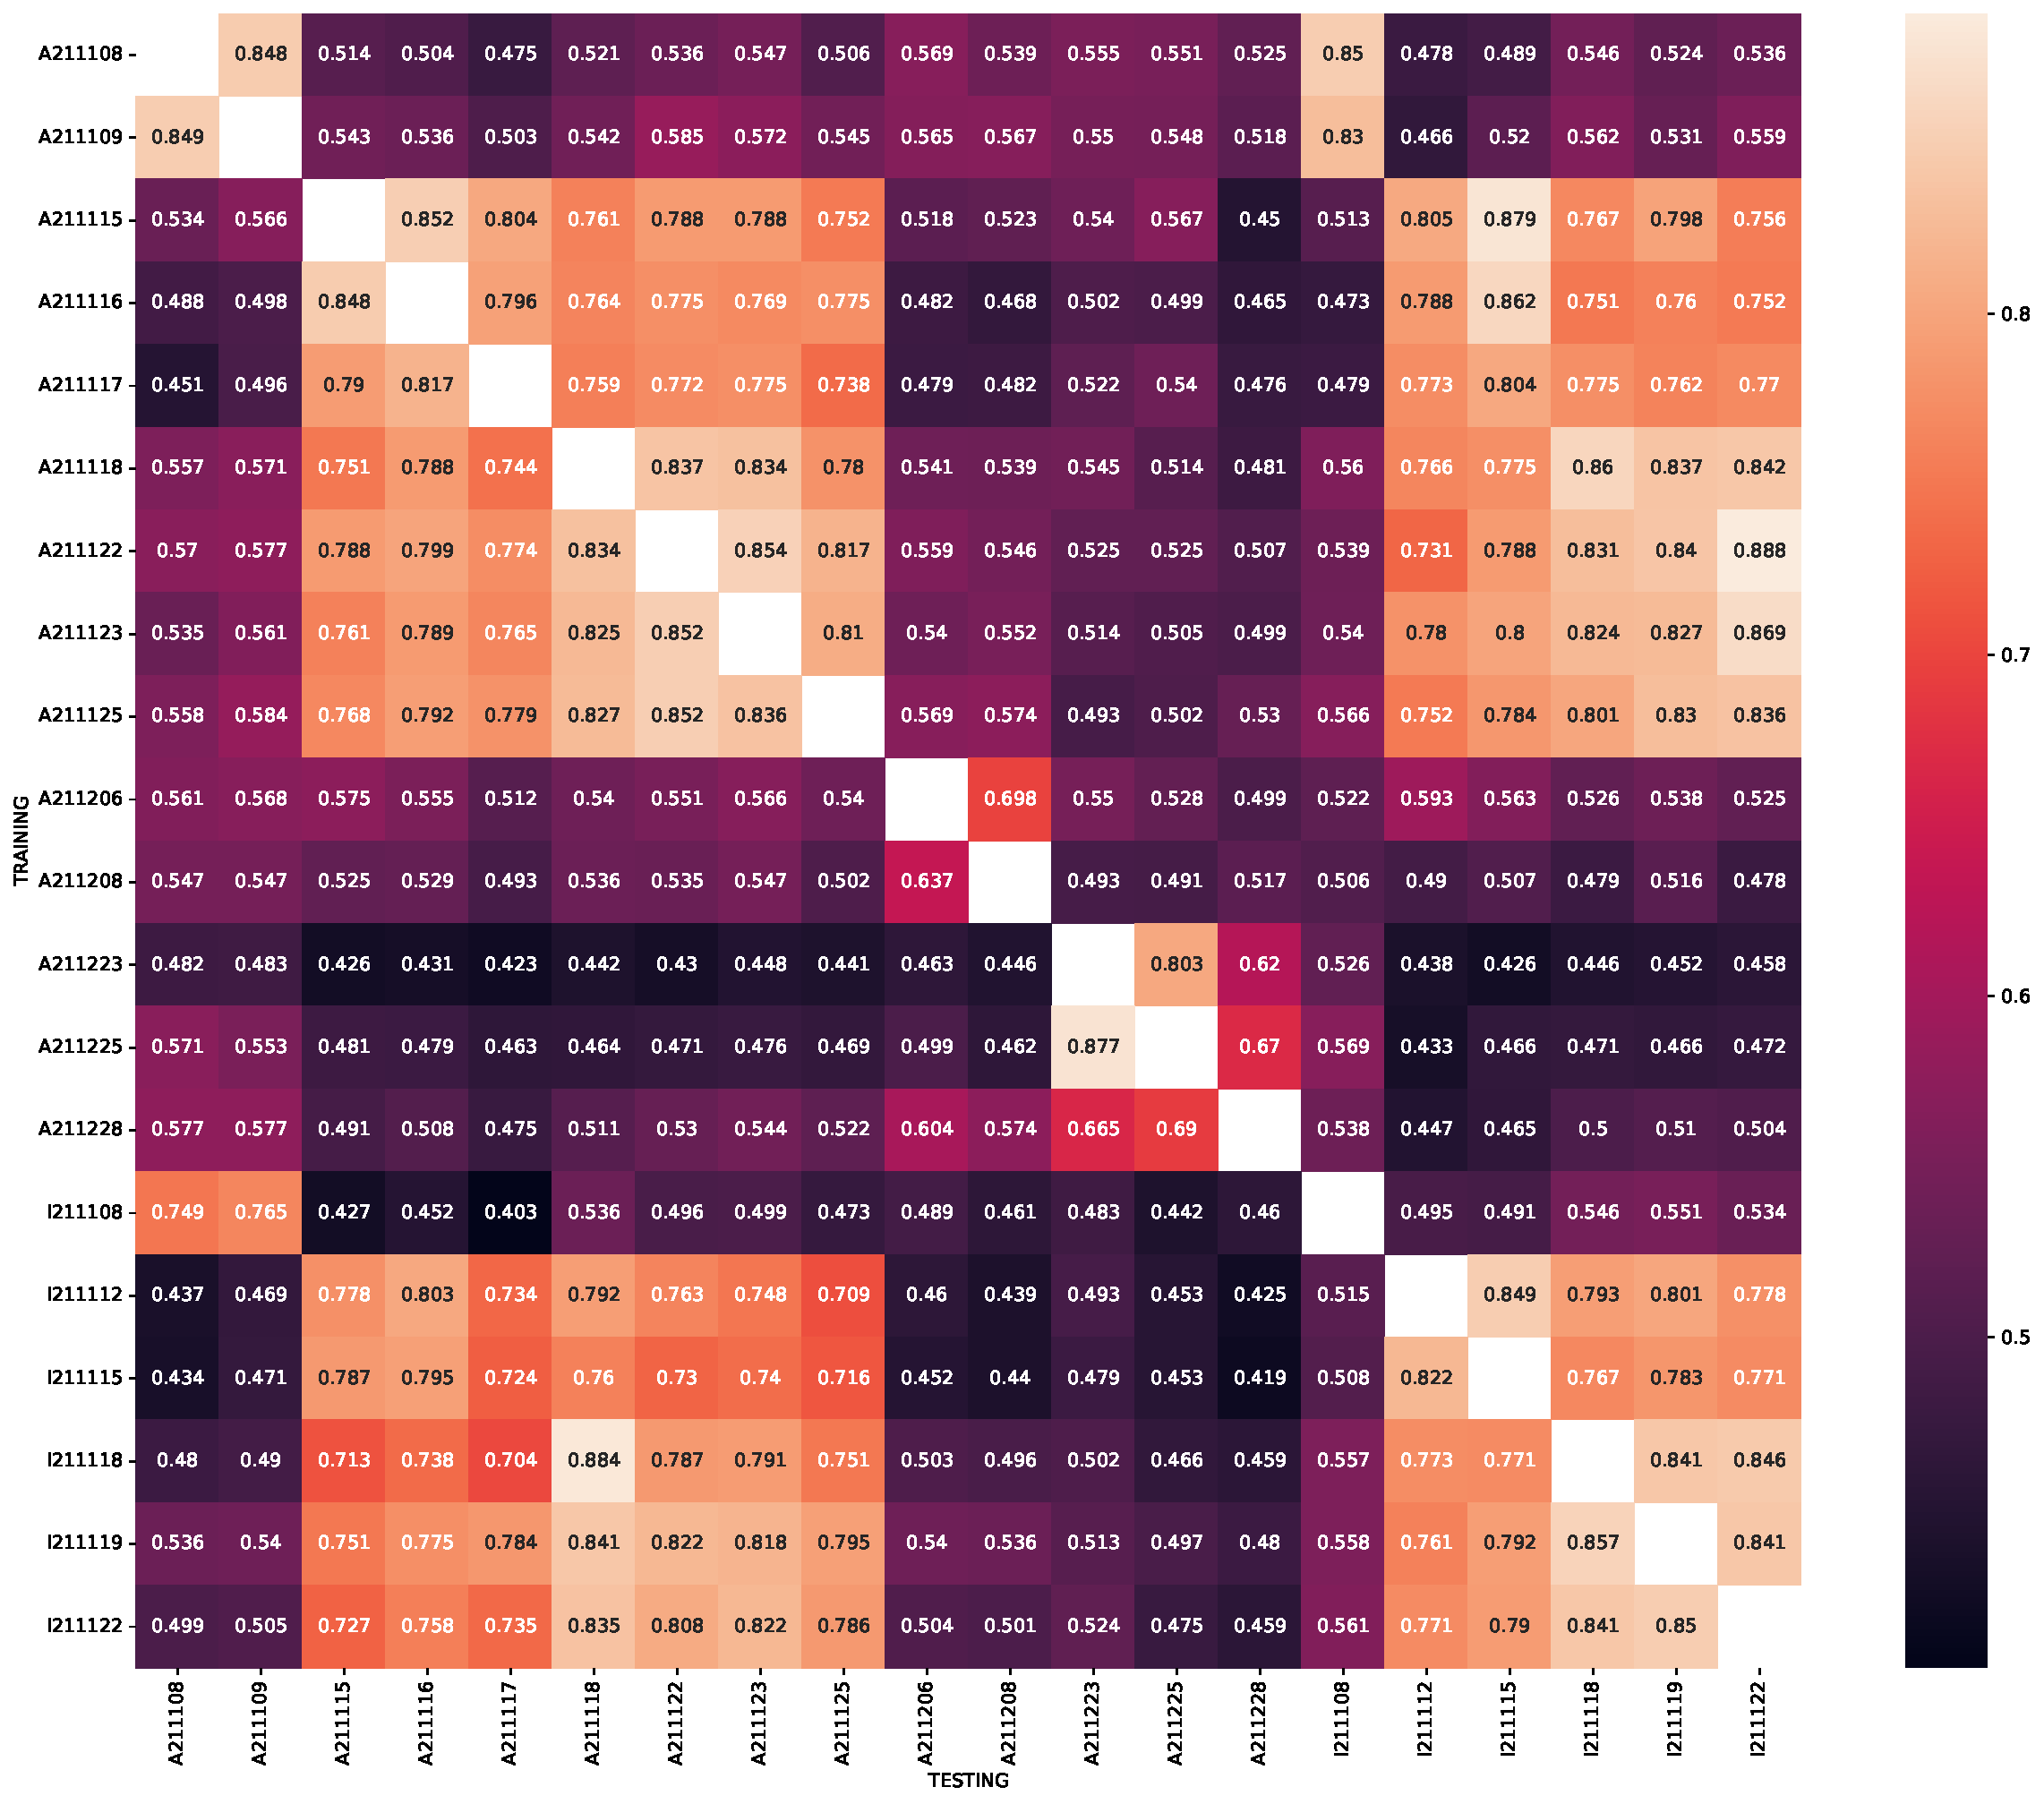
\includegraphics[width=85mm]{images/cm2.pdf}}}\\
	\subfloat[\label{fig:comp_2}\centering ]{{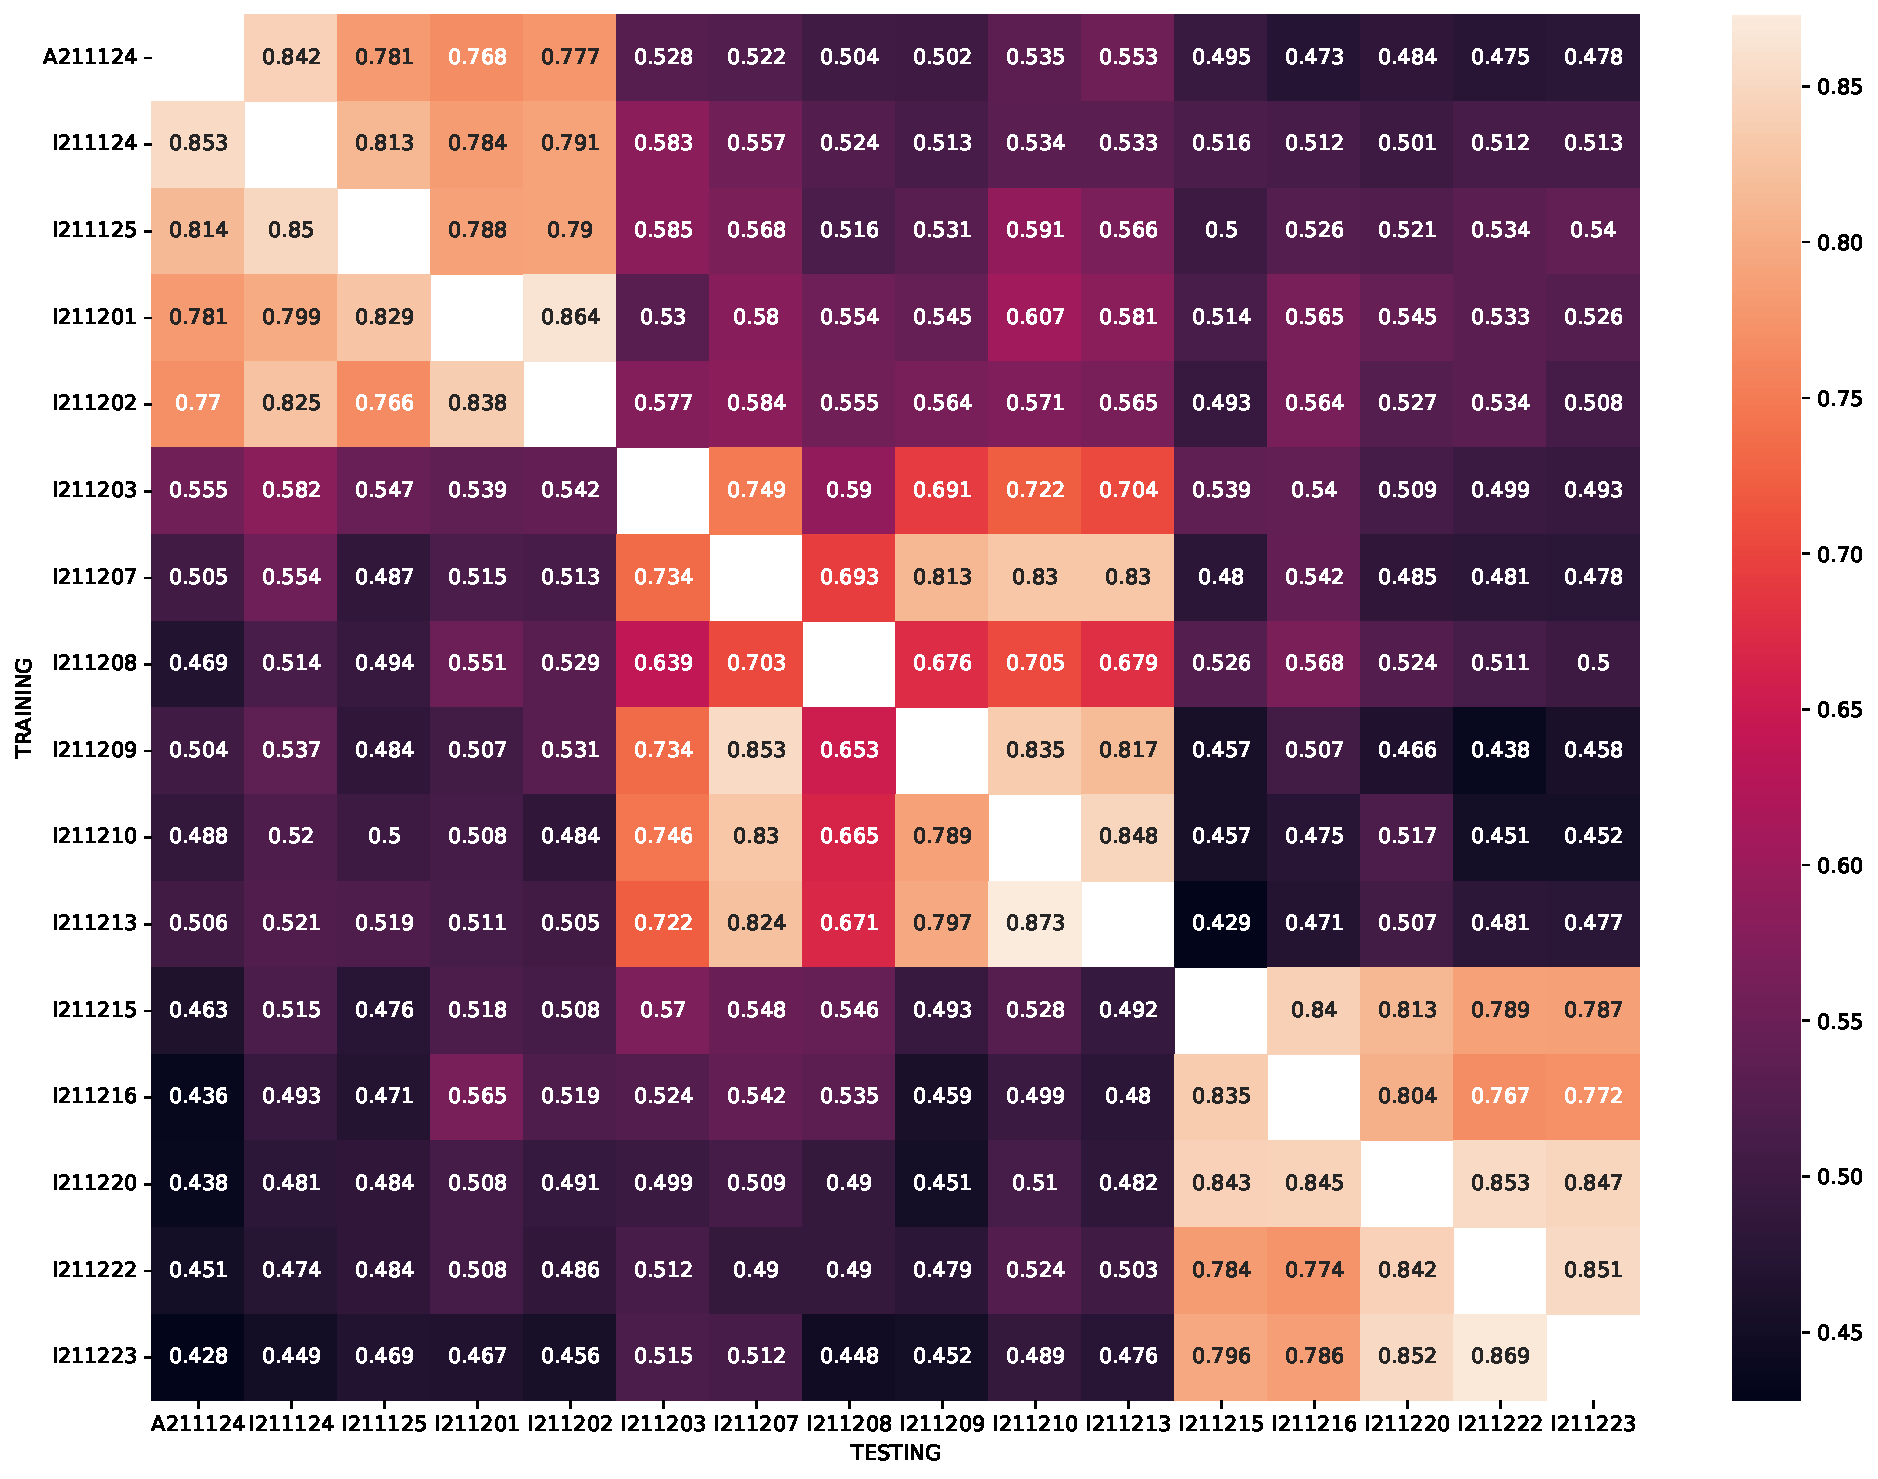
\includegraphics[width=85mm]{images/cm4.pdf}}}%
	
	
	\caption{F1 scores of sessions pairs  assigned as training and test sets.}
	\label{fig:stepsofID}
\end{figure}



These results reflect overall success. In total, we made more than 600 session pair comparisons. In these comparisons, the first session of the pair was used as training and the second as testing. If we divide these sessions into active and idle, four different possibilities are possible Active vs Active  (AA), Active vs Idle  (AI), Idle vs Active  (IA), and  Idle vs Idle  (II). In this context, the distribution of session comparisons is given in Fig.~\ref{fig:pie}.  
\begin{figure}[ht]
	%	\vspace*{-3mm}
	\centerline{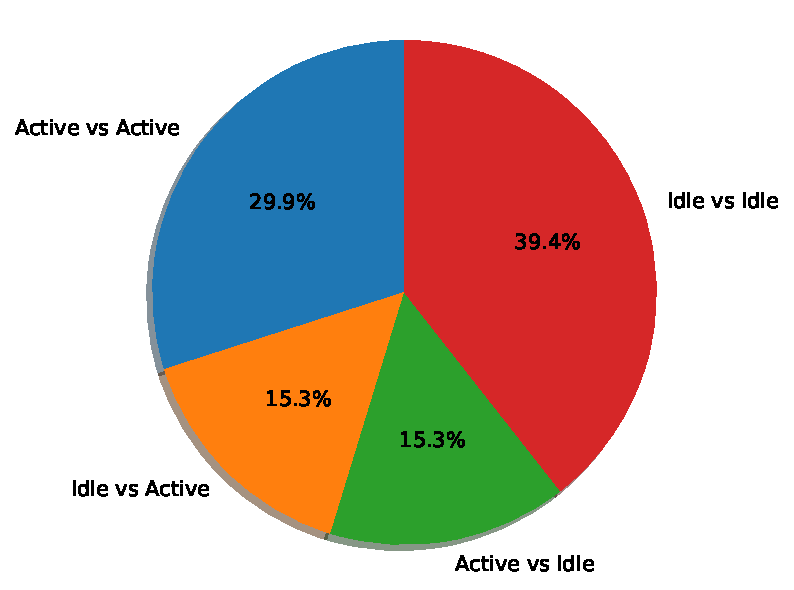
\includegraphics[width=0.61\columnwidth]{images/pie.pdf}}
	\caption{The number of packets produced by the devices in the Aalto dataset.}
	\label{fig:pie}
\end{figure}


We believe that focusing on class/device-based results will give more information. By analysing the device-based results for each session, we want to focus on the problematic devices. In this context, a device that is unsuccessful in any of the sessions, with a class-based F1 score of less than 0.50, is added to our list if it repeats this behaviour more than 12 times in all comparisons (12 corresponds to 2\% of all session comparisons). Fig.~\ref{fig:bar}.  shows this list. The list shows the number of times the device class has failed and the distribution of these failures according to the session benchmark types.


Examining Fig.~\ref{fig:bar}, we can see that, with some minor exceptions, the overall distribution of the pie chart remains the same. This shows that there is no significant difference between idle and active. On the other hand, if we focus on some devices with low performance, we can easily understand why they are included in the list. The devices with the highest number of failures are those with more than one example in the experimental set, such as Amazon Alexa Echo Dot, Gosund Plug, Gosund Socket, Teckin Plug, Yutron Plug. Since these devices are different examples of the same device (same brand and model), they should be grouped under one label (e.g. Teckin Plug 1 and Teckin Plug 2 -> Teckin Plug). We believe that the success level of most of the other devices can be improved by increasing the sample diversity. In this context, we aimed to increase the sample diversity by taking samples from multiple sessions and, as a consequence, to increase the model success.
In this context, we separated all sessions into two parts, training and test sessions, in such a way that the sessions are isolated from each other. By combining the sessions that we determined as training and test, we obtained a very large dataset. While creating this dataset, we isolated idle and active data in their own types. We obtained 2 pairs of datasets, idle training and testing consisting only of idle data, and active training and testing consisting only of active data. However, we took the data of D-Link Water Sensor, a device not included in the active sessions, from the idle sessions. Another change was related to LG Smart TV device. The data for this device is only present in three of the 54 sessions. However, the data for this device is so unbalanced that the device data collected from only 3 out of 54 sessions account for about 9\% of the total number of packets in all 40 devices. We removed this device from the dataset both because it did not have data from enough sessions and because its excessive number of packets distorted the distribution of the dataset.



In order to obtain a dataset that reflects the diversity of the sessions but is not too large, we reduced the number of packets in these 4 datasets to 10\% of the total number of packets per dataset. Since we used random samples during this process, the packet rates obtained from the devices remained constant so that we did not damage the natural distribution of the dataset.


The comparison of the 4 different cases in terms of F1 score is given in the graph.



\begin{figure*}[ht]
	%	\vspace*{-3mm}
	\centerline{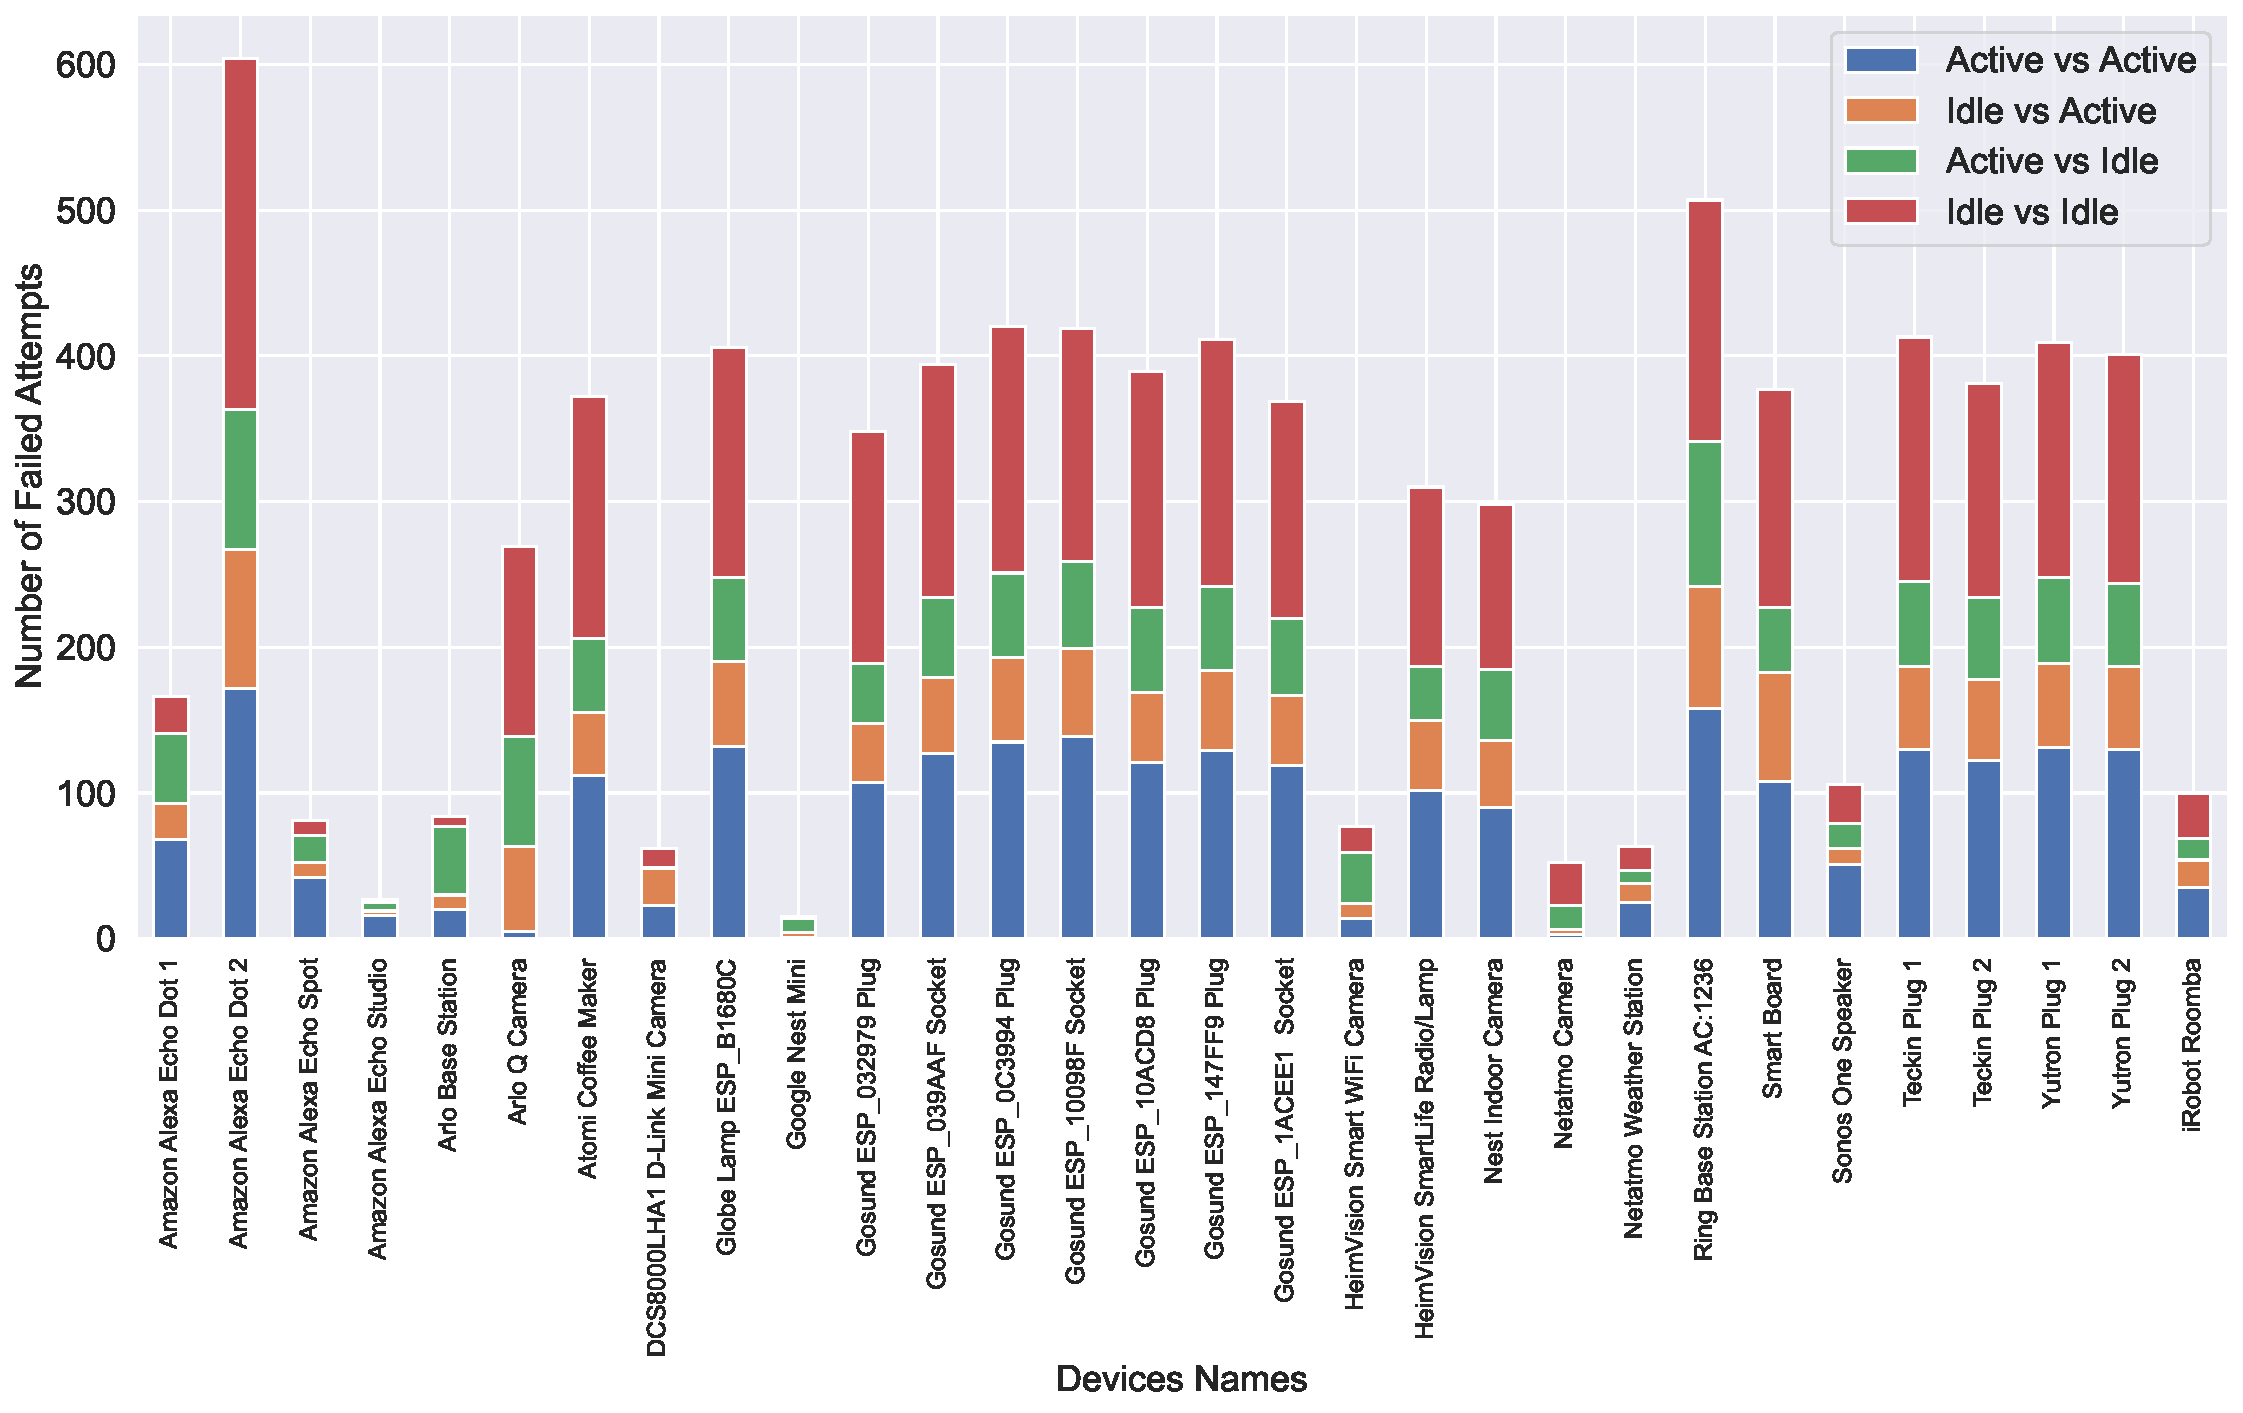
\includegraphics[width=1.7\columnwidth]{images/bar.pdf}}
	\caption{The number of packets produced by the devices in the Aalto dataset.}
	\label{fig:bar}
\end{figure*}

\begin{figure}[ht]
	%	\vspace*{-3mm}
	\centerline{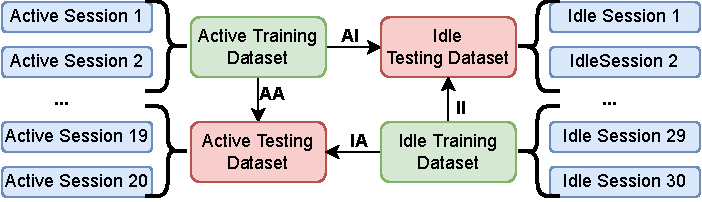
\includegraphics[width=1\columnwidth]{images/data.pdf}}
	\caption{The number of packets produced by the devices in the Aalto dataset.}
	\label{fig:bar}
\end{figure}


















% Table generated by Excel2LaTeX from sheet 'Sheet1'
\begin{table}[htbp]
	\centering
	\caption{Add caption}
	\begin{tabular}{@{}clllrrr@{}}
		\toprule
		& Data  & Accuracy & F1Score & \multicolumn{1}{l}{Train-t} & \multicolumn{1}{l}{Test-t} & \multicolumn{1}{l}{Al-time} \\
		\midrule
		\multirow{4}[2]{*}{\begin{sideways}Individual\end{sideways}} & AA    & 0.890±0.001 & 0.842±0.004 & 1.748 & 0.204 & 0 \\
		& AI    & \underline{0.918±0.001}  & \underline{0.905±0.005} & 1.812 & 0.287 & 0 \\
		& IA    & 0.823±0.046 & 0.818±0.015 & 1.699 & 0.223 & 0 \\
		& II    & 0.821±0.004 & 0.814±0.007 & 1.721 & 0.291 & 0 \\
		\midrule
		\multirow{4}[2]{*}{\begin{sideways}Aggregated\end{sideways}} & AA    & 0.943±0.001 & 0.925±0.007 & 1.962 & 0.235 & 9.119 \\
		& AI    & \underline{0.999±0.000} & \underline{0.999±0.000} & 1.864 & 0.299 & 11.519 \\
		& IA    & 0.850±0.058 & 0.898±0.017 & 1.584 & 0.206 & 8.46 \\
		& II    & 0.904±0.004 & 0.912±0.006 & 1.630  & 0.313 & 11.267 \\
		\bottomrule
	\end{tabular}%
	\label{tab:result}%
\end{table}%






% Table generated by Excel2LaTeX from sheet 'Sheet1'
\begin{table}[htbp]
	\centering
	\setlength{\tabcolsep}{3pt}
	\caption{Add caption}
	\begin{tabular}{@{}lrrrrrrrr@{}}
		\cmidrule{2-9}          & \multicolumn{4}{c}{Individual}
		& \multicolumn{4}{c}{ Aggregated} \\
		\midrule
		& \multicolumn{1}{c}{AA} & \multicolumn{1}{c}{AI} & \multicolumn{1}{c}{IA} & \multicolumn{1}{c|}{II} & \multicolumn{1}{c}{AA} & \multicolumn{1}{c}{AI} & \multicolumn{1}{c}{IA} & \multicolumn{1}{c}{II} \\
		\midrule
		Amcrest WiFi-Cam. & 0.968 & 0.979 & 0.951 & 0.959 & 0.992 & 1.000 & 1.000 & 1.000 \\
		Amazon AE Dot & 0.933 & 0.938 & 0.950 & 0.947 & 0.997 & 1.000 & 0.998 & 1.000 \\
		Amazon AE Spot & 0.555 & 0.838 & 0.844 & 0.837 & 0.559 & 1.000 & 0.999 & 0.999 \\
		Amazon AE Studio & 0.821 & 0.874 & 0.837 & 0.736 & 0.981 & 1.000 & 0.999 & 0.979 \\
		Amazon Plug & 0.995 & 0.999 & 0.997 & 0.999 & 1.000 & 1.000 & 1.000 & 1.000 \\
		Arlo Base Station & 0.984 & 0.819 & 0.624 & 0.864 & 1.000 & 0.998 & 0.454 & 1.000 \\
		Arlo Q Camera & 0.987 & 0.970 & 0.969 & 0.952 & 1.000 & 1.000 & 1.000 & 1.000 \\
		Atomi Coff-Maker & 0.847 & 0.892 & 0.890 & 0.501 & 0.999 & 1.000 & 1.000 & 0.638 \\
		Borun Camera & 0.982 & 0.981 & 0.972 & 0.978 & 0.999 & 0.999 & 0.999 & 0.999 \\
		D-Link Mini Cam. & 0.982 & 0.989 & 0.342 & 0.906 & 1.000 & 1.000 & 0.756 & 1.000 \\
		D-Link Water Sen. & 0.930 & 0.936 & 0.936 & 0.934 & 1.000 & 0.989 & 1.000 & 0.989 \\
		Eufy HomeBase 2 & 0.815 & 0.812 & 0.782 & 0.806 & 1.000 & 0.998 & 1.000 & 0.998 \\
		Globe Lamp  & 0.654 & 0.823 & 0.916 & 0.431 & 0.900 & 0.997 & 1.000 & 0.246 \\
		Google Nest Mini & 0.975 & 0.971 & 0.952 & 0.879 & 1.000 & 1.000 & 0.996 & 0.982 \\
		Gosund Plug & 0.839 & 0.899 & 0.917 & 0.706 & 0.968 & 0.995 & 0.999 & 0.724 \\
		Gosund Socket & 0.868 & 0.893 & 0.895 & 0.532 & 0.992 & 0.995 & 0.999 & 0.406 \\
		HeimVision S Cam. & 0.986 & 0.998 & 0.934 & 0.984 & 1.000 & 1.000 & 1.000 & 1.000 \\
		HeimVision Lamp & 0.715 & 0.838 & 0.857 & 0.518 & 0.965 & 0.999 & 1.000 & 0.759 \\
		Home Eye Camera & 0.930 & 0.911 & 0.927 & 0.910 & 1.000 & 1.000 & 1.000 & 1.000 \\
		Luohe Cam Dog & 0.762 & 0.760 & 0.759 & 0.757 & 1.000 & 0.995 & 1.000 & 0.994 \\
		Nest Indoor Cam. & 0.998 & 0.997 & 0.999 & 0.910 & 0.999 & 0.999 & 1.000 & 0.997 \\
		Netatmo Camera & 0.969 & 0.986 & 0.398 & 0.934 & 1.000 & 1.000 & 0.381 & 1.000 \\
		Netatmo Weather & 0.826 & 0.827 & 0.868 & 0.845 & 1.000 & 1.000 & 1.000 & 1.000 \\
		Philips Hue Bridge & 0.994 & 0.990 & 0.978 & 0.986 & 1.000 & 1.000 & 1.000 & 1.000 \\
		Ring Base Station & 0.305 & 0.913 & 0.293 & 0.697 & 0.336 & 1.000 & 0.250 & 0.995 \\
		SIMCAM 1S & 0.996 & 0.998 & 0.980 & 0.998 & 1.000 & 1.000 & 1.000 & 1.000 \\
		Smart Board & 0.363 & 0.721 & 0.292 & 0.675 & 0.105 & 0.996 & 0.074 & 0.996 \\
		Sonos One Speaker & 0.729 & 0.844 & 0.727 & 0.891 & 0.991 & 0.999 & 0.951 & 1.000 \\
		Teckin Plug & 0.675 & 0.826 & 0.868 & 0.578 & 0.932 & 1.000 & 1.000 & 0.712 \\
		Yutron Plug & 0.764 & 0.855 & 0.867 & 0.632 & 0.956 & 1.000 & 1.000 & 0.850 \\
		iRobot Roomba & 0.955 & 0.962 & 0.843 & 0.946 & 1.000 & 1.000 & 0.993 & 1.000 \\
		\midrule
		Mean  & 0.842 & 0.905 & 0.818 & 0.814 & 0.925 & 0.999 & 0.898 & 0.912 \\
		\bottomrule
	\end{tabular}%
	\label{tab:addlabel}%
\end{table}%











\clearpage

An IoT device is any item that has a unique identity that can connect to other devices and perform control commands\cite{al2015internet}. It is a bridge that connects our cyber world and our physical world\cite{patel2018internet}. Using IoT, we can manage our physical world from our cyber world.

This rapid progress has enabled many of us to include IoT devices in our lives. However, as a result of this rapid progress, many IoT devices were launched by many different manufacturers in a very short time. This rapid progress brings to mind the issue of whether devices are safe or how to ensure their safety.


It is unlikely to apply the solutions applied to classical computers to IoT devices. Because most of these devices have very limited possibilities in terms of battery, processor and storage. Also, due to the heterogeneous nature of IoT, there is no standard among these devices. Many use a unique operating system and hardware. In addition, IoT devices do not have the standard interfaces as conventional computers. This situation limits user-device interaction. In today's world, where there are a wide variety of devices, users can't take the security measures that every device needs. IoT device identification is a method that aims to find the device identity, such as brand and model, by analyzing the device behaviour.

Thanks to this method, devices on the network can be detected, and the necessary security measures can be taken for these devices. For example, the software of the needed ones can be updated, the behaviour of the devices and the addresses they will connect to can be restricted, or these devices can be isolated from the rest of the network. 

In this study, we have divided the device identification process into four steps (see Figure~\ref{fig:stepsofID} ), and included possible mistakes to be made in each step and how to deal with these mistakes.

Parallel to these steps, the structure of the paper is as follows.
In Section~\ref{section:Methods}, device identification methods are discussed. Section~\ref{section:data} examines data types and considerations when choosing the appropriate dataset. Section~\ref{section:Features}  highlights the feature extraction step and its key points. Section~\ref{section:ML}   discusses how to decide on the appropriate machine learning method. In Section~\ref{section:Evaluation}  , evaluation methods and their pros and cons are explained.


%The paper is organised as follows.  reviews related work. Section~\ref{section:Materials and Methods} describes the methods we use to model network packets, and the data sets used for evaluation. Section~\ref{section:Model Selection} gives an overview of our model selection approach, Section~\ref{section:Performance Evaluation} evaluates the selected model, and Section~\ref{section:Performance Comparison} compares it against other DI approaches. Limitations are discussed in Section~\ref{section:Limitations}, and conclusions are presented in Section~\ref{section:Conclusion}.





\section{Familiarizing with Methods}\label{section:Methods}

In this section, different device identification methods are introduced and their advantages and disadvantages are discussed.

%\noindent\textbf{Decide what to classify}
\subsection{Define the limits of the scope of the IoT concept you will use in your study.}
The Internet of Things (IoT) can be defined as all physical objects that can share data with other devices, have embedded sensors, software and various technologies~\cite{hussain2020machine}. However, this definition is too general. For your own work, you must decide what to consider as IoT and define the boundaries of your definitions. For example, if your data will contain, will you collect classic computers or mobile devices such as tablets and phones or routers and switches under this definition or will you consider them as non-IoT devices? Will you accept Wireless Sensor Network (WSN) devices as IoT or will you create a separate subgroup for them? When classifying IoT devices, will you focus on a certain sub-area (home type, smart cities, agriculture, army, etc.\@).

\subsection{Consider different methods of device identification.}
Deciding what kind of definition you will make is very important as it will affect other steps of your work. You can  identify according to devices with 3 different approaches~\cite{yadav2020position}:
\textbf{Unique Identification:} By accepting each of the devices as unique, a separate class is created for each device~\cite{hamad2019iot}.\\
\textbf{Type Identification:}  Identification is performed according to the device type. If there are multiple devices of the same make and model, they are seen as a single class~\cite{miettinen2017iot}.\\
\textbf{Class Identification:}  Different devices that are not the same but have similar features, e.g., produced by the same brand for similar tasks, are gathered under a single class~\cite{nguyen2019diot,aksoy2019automated}.

\begin{figure}[ht]
	%	\vspace*{-3mm}
	\centerline{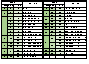
\includegraphics[width=1\columnwidth]{images/tablo3.pdf}}
	\caption{Labelling the Aalto dataset according to 3 identification approaches.}
	\label{fig:comparedata}
\end{figure}


Fig.~\ref{fig:comparedata} shows the labelling of the Aalto University IoT Devices Captures 
dataset~\cite{aalto2017dataset} with three viewpoints. In the dataset containing 33 devices in total, 33 different labels are formed in the unique method, 27 different labels in the type method, and 15 different labels in the class method. Which of these three perspectives you choose is also effective in determining the network traffic characteristics you will use in your design. 

\subsection{Remember that using flow-based or packet-based features affects the generalizability of your models.}
In your design, you can use packet-based, flow-based features or both. However, if you use Unique Device Identification, the features you will only get from the packets will not be enough.  you will also need to use the flow-based features. On the other hand, using flow features will reduce the generalizability of your model, resulting in your model being specific only to the design you are using. 

\subsection{Analyze the strengths and weaknesses of these methods and choose according to your needs.}
Type Identification and Class Identification methods allow you to obtain a model with higher generalizability by using only packet-based features. Using the Type Identification method does not promise great success in distinguishing similar devices, because similar devices show similar behavior patterns. Against this disadvantage, Class Identification can be used, which gathers similar devices under the same label. This approach is based on the assumption that similar devices can be grouped under the same group because they have similar hardware and software. However, in this method, expert involvement is required to decide on the similarities and groups of the devices. Before deciding on the method you will use in your design, it will be appropriate to examine the advantages and disadvantages of these methods, and to decide according to your purpose.

\section{Familiarizing with Data}\label{section:data}
In this section, how the data you will use can be obtained, the characteristics and qualities that the data should have are examined.

\subsection{Decide how you will obtain the data.}

One of the important steps in device identification studies is how to obtain the data. In this context, you can use simulation or real devices. Although using simulation is fast, cheap, and easy, simulation programs currently lack the ability to simulate the various types of IoT devices because of the extremely heterogeneous nature of IoT devices. Therefore, the use of simulation is mostly seen in studies where many homogeneous devices such as WSN are used.


\subsection{Do not forget about privacy if you are using real data.}
In the use of real IoT devices, there are options to create an experiment set or usage of real data. When using test sets it is important that the devices can mimic as much as possible  usage patterns. Although using real data may seem advantageous in many ways, the danger of causing privacy disclosures should be considered. If you are collecting data from a real environment, you should consider the ethical aspect, obtain the necessary relevant permissions and censor any information that may disclose confidentiality such as user identity or IP addresses.

\subsection{Use data from previous studies.}
Another data acquisition method is the use of other previously collected publicly available data. The use of such data is very advantageous as it does not require extra cost and provides the results to be comparable with the literature. You can scan the literature to find the appropriate data set, especially survey studies on device identification and fingerprinting can be very useful. You can also use websites specialized for datasets, e.g.,~\href{https://datasetsearch.research.google.com/}{Dataset Search},~\href{https://www.kaggle.com/datasets}{Kaggle}, and~\href{https://archive.ics.uci.edu/ml/datasets.php}{UCI ML Repository}


\subsection{Unsure the data is  suitable and has the  necessary qualifications.}

In addition, no matter how you obtain your data, the data you will use for device identification must have the following characteristics:

\begin{itemize}
	\item It should contain benign data. In device identification, you need to extract the behavior patterns of the devices. For this, you need the normal/benign data of the devices. However, if the benign and malicious  data packets are separated, you can also use the normal parts of the data sets prepared for anomaly detection (e.g.,~\href{https://iotanalytics.unsw.edu.au/attack-data}{UNSW IoT benign and attack traces~\cite{UNSW2018attack}}). Another point that can be overlooked is that the tools used in vulnerability testing are very similar to attack tools. You can classify the data obtained by performing vulnerability tests on them as attack data, not normal data.

	\item The dataset should contain enough data. It is essential for a robust study that the dataset contains as many and varied devices as possible. In this way, the operation of your model is observed more soundly and the probability of success by chance is reduced.
	
	\item Devices must be labelled. In the dataset you will use, you should know which device the packets belong to (which device was produced by).
\end{itemize}


\subsection{Ensure that the correct labels are assigned to the data.}

It is quite common to use MAC and IP addresses to identify  devices, but care should be taken when using these addresses. Especially if there are Non-IP devices in the datasets, this information can be misleading. The Aalto dataset is a good example for this.  The non-IP HueSwitch device is connected to the gateway where data collection is made, via the HueBridge device. The HueSwitch transmits the network packets to the HueBridge device using ZigBee, which then HueBridge re-encapsulates these network packets and forwards them to the gateway via Ethernet. HueSwitch packets arriving at gateway carry the MAC addresses of the HueBridge device, not their own MAC addresses. Therefore, HueBridge and HueSwitch devices are represented by a single MAC address in the Aalto dataset. So, MAC and IP addresses cannot be used for labelling.  That's why the creator of the dataset labelled the devices separately.

\subsection{Remember that IoT devices are highly heterogeneous and this affects data distribution.}
IoT devices are tools that contain a wide variety of software and hardware, produced for many different purposes. This is why data from devices can be quite diverse. So, IoT devices have an unbalanced data distribution due to their highly heterogeneous nature. One device in a network can generate a large amount of data, while another device can generate a very small amount of data. Fig.~\ref{fig:aalto} shows the number of packets produced by the devices in the Aalto dataset. 

\subsection{Use data augmentation  to deal with scarce data.}
This unbalanced distribution of data can negatively affect some machine learning methods. You can deal with this problem by using data augmentation techniques. The most important point during this process is to isolate the test and training datasets from each other \textbf{before} data augmentation. In this way, the augmented (post-generated) data in the training dataset is prevented from leaking into the test data.


\subsection{Protect test data from all influence}
Another common mistake is to apply augmentation of test data. It is best to keep the test data in its original state. Even the simple process of resampling, such as copying packets, is harmful because it will break the distribution of test data. The distribution of  test dataset should also show the true world distribution. Thus, you can evaluate the outputs of your model more realistically and check whether there is a real contribution on data augmentation.

\begin{figure}[ht]
	%	\vspace*{-3mm}
	\centerline{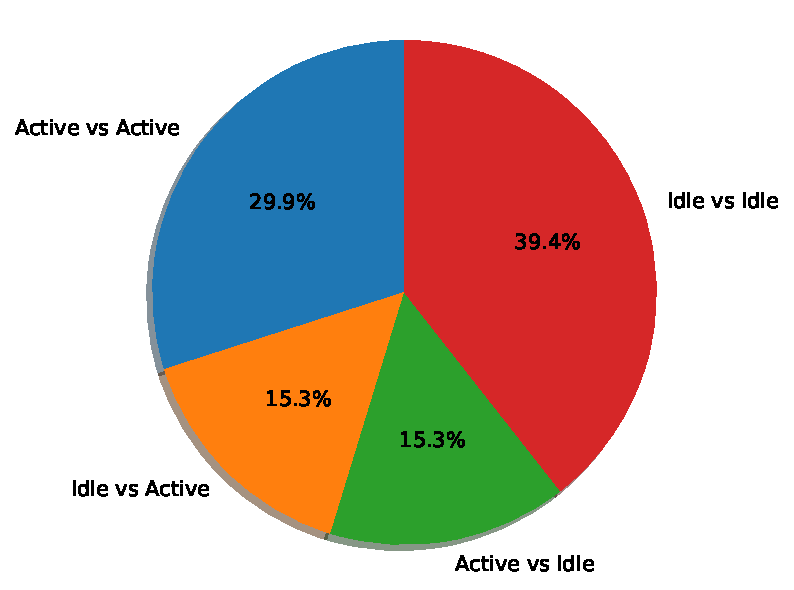
\includegraphics[width=1\columnwidth]{images/pie.pdf}}
	\caption{The number of packets produced by the devices in the Aalto dataset.}
	\label{fig:aalto}
\end{figure}




\section{Familiarizing with Features Extraction}\label{section:Features}
In this section, the feature extraction process and important points to be considered during this process are highlighted.

\subsection{Save time by choosing the right tools for preliminary analysis.}

One disadvantage of working with network data is dealing with huge amounts of data. Analysing this data and extracting features can be very time consuming. Therefore, it is very important to choose the right tools for these operations. Recently, python-based libraries such as ~\href{https://dpkt.readthedocs.io/en/latest/}{dpkt} and ~\href{https://scapy.net/}{scapy} have been used extensively in the analysis of pcap data and feature extraction. Note that although they are easy to use and supported by a lot of documentation, they are extremely slow. Especially in very large data, using C-based programs such as ~\href{https://www.wireshark.org/}{Wireshark} for your pioneering analysis will save you time. Even, with ~\href{https://www.wireshark.org/docs/man-pages/tshark.html}{tshark}, which you can automate with bash code, you can do many operations much faster.

\subsection{Avoid features that uniquely identify your device.}
Get to know the features you will use during the feature extraction process. Avoid including passive features such as MAC and IP addresses in your feature set. These properties are identifying features. They uniquely identify devices but do not provide any information about device behaviour. Even if you get high results using these features in your experiments, these results cannot be generalized because they suffer from overfitting.
\subsection{Avoid features that uniquely identify a session.}
Some session-based features are highly identifying, despite not static. However, these features uniquely identify the session, not the device. For example, various features such as port numbers, IP ID, TCP sequence numbers are determined at the beginning of the session, and are used until the session ends. Because these properties are randomly determined, they are not predictable or generalizable. You can avoid using these features in your study. If you are going to use it, you can do it in a healthy way. For example, isolate the test and train datasets from each other to ensure that they consist of different sessions. Thus, you can prevent these features, which are identifying for each session, from leaking from the training data to the test data.

\subsection{Beware of features  that are implicitly identifying.}  Although time-related features such as timestamps do not appear to be stand-alone identifying, they can be identifiers as they will uniquely show a device's operating timespan. Header checksum features are another example of this situation. Checksum features are a summary of the header in which they are used. So IP checksum contains information about IP addresses, TCP checksum contains sequence,  acknowledgment  numbers, UDP checksum  contains  port numbers.  If you find it inconvenient to use any attribute in the header, you should also avoid using the header's checksum feature.

\begin{figure}[ht]
	%	\vspace*{-3mm}
	\centerline{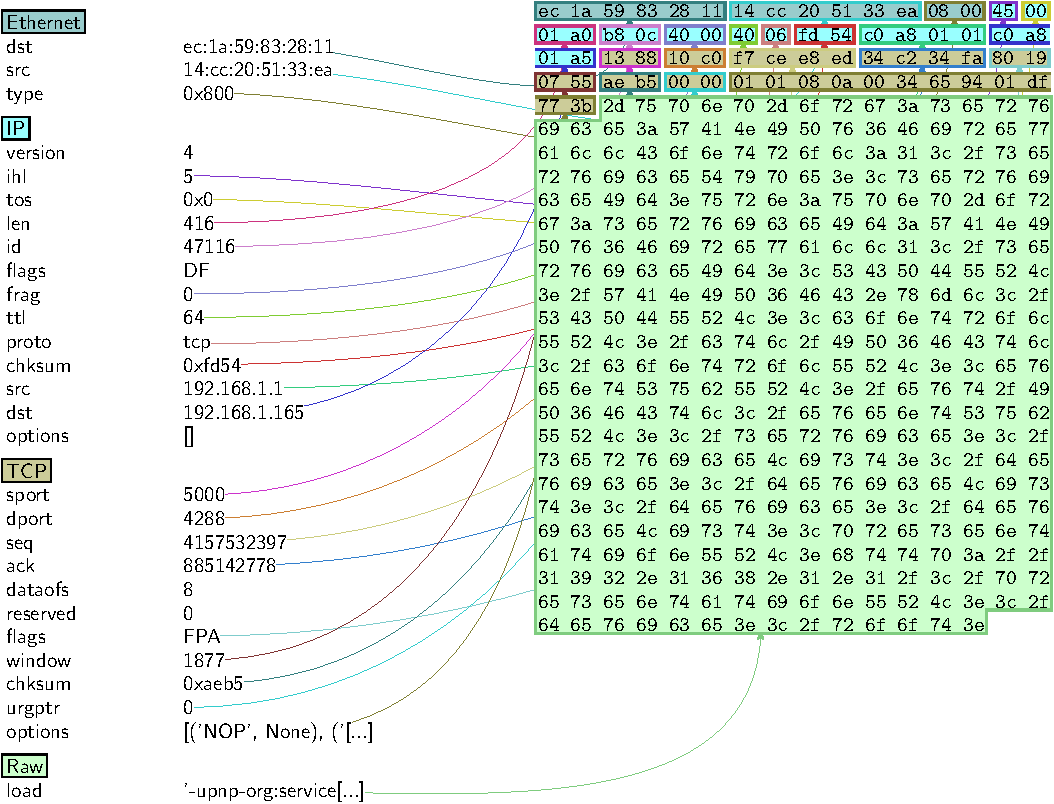
\includegraphics[width=1\columnwidth]{images/bytes.pdf}}
	\caption{The fields contained in a network packet and their byte equivalents..}
	\label{fig:bytes}
\end{figure}

\subsection{Be careful when extracting features from raw data.}
An alternative method in the feature extraction stage is the use of raw bytes. This method is based on obtaining feature sets through various size reduction methods by converting network data into raw bytes.  A network packet converted to raw bytes is given in Fig.~\ref{fig:bytes}. This method is advantageous in terms of both obtaining original features and reducing expert involvement in the feature extraction stage. There is no harm in using this method in the packet payload, but if you include the packet headers, you may leak many features that you would not normally want to use in the feature set. So, when applying this method, it should be noted that raw data contains identifying features. Therefore, before performing feature extraction, censoring the raw data corresponding to the identifying features ensures that more robust features are extracted, and prevents errors that would lead to overfitting.



\section{Familiarizing with Machine Learning}\label{section:ML}
In this section, it is focused on what should be considered when using machine learning methods and how the methods can be selected.

\subsection{Consider other options when creating a multiclass model.}
Device identification is a multi-class problem. However, there are some disadvantages of using multi-class models in solving this problem. The multi-class approach makes it difficult to extend the model. Because every time a new device is added to your system, you will have to retrain the model. In addition, scalability issues may arise as the number of devices increases. One2all approach can be preferred to deal with this problem. In this approach, a separate binary model is created for each device, and a multi-class result is obtained from the outputs of these models. In case a new device is included in this system, there is no need to recreate the whole models, only the model of this new device is added.

\subsection{Do not underestimate the classical ML approaches}
Do not underestimate the classical/older approaches when choosing the ML method you will use. Although deep learning methods have been popular recently, it has been observed that classical methods such as decision trees are much more successful than deep learning methods, especially in evaluating tabular data that lack temporal relationships, such as device identification~\cite{lundberg2020local2global}. 

\subsection{Consider the interpretability of the models}
Interpretability of algorithms can also be a matter of preference. Methods such as liner/logistic regression, DT, kNN have a high level of interpretability, while SVM, Ensemble methods and deep learning have a low level of interpretability (see Fig.\ref{fig:interpretability}). High interpretability can be very useful when analysing and evaluating features~\cite{arrieta2020explainable}.
\begin{figure}[ht]
	%	\vspace*{-3mm}
	\centerline{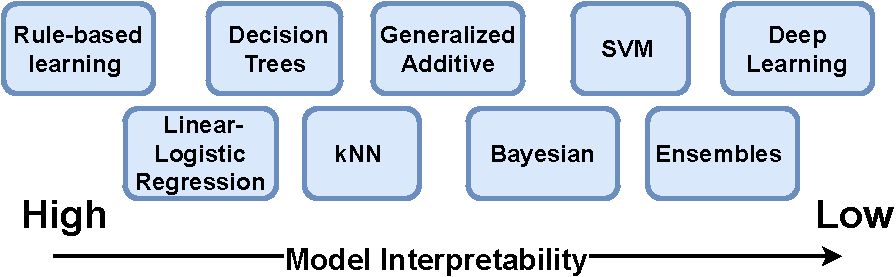
\includegraphics[width=1\columnwidth]{images/ModelInterpretability.pdf}}
	\caption{Interpretability levels of some machine learning methods.}
	\label{fig:interpretability}
\end{figure}
\subsection{Note that there is no free lunch.}
There is no perfect machine learning method that works best on every data type\cite{wolpert2002supervised}. Try to find the appropriate machine learning method for your data. With so many methods available, finding the best method can be costly. You can try different strategies for this. For example, taking a look at the methods used by similar previous studies can be very helpful, especially survey studies. Another method would be to try one of each type of machine learning (for example, tree-based, kernel-based, ANN-based etc.) and experiment more deeply with the type that performs best.


\subsection{Consider the success - inference time trade-off.}
Do not accept detection success as the only criterion. In network technology, transactions are done at the micro-milliseconds level. The fast sorting capability of your model, which will be used in the real world and will work in a critical area such as security, is as important as the correct classification capability. Although some algorithms such as SVM and kNN achieve high performance levels, their inference time can be very high. Therefore, it is highly recommended to include the inference time criterion in your evaluation and to avoid algorithms with very high inference times.



\section{Familiarizing with Evaluation}\label{section:Evaluation}
In this section, performance evaluation methods are examined and their pros and cons are discussed.


\subsection{Consider data distribution when choosing the evaluation method.}
Various evaluation criteria are used to see how successful the study is. Accuracy is the most popular of these criteria. Since it is used for evaluation in many studies, using accuracy will add comparability to your study. However, in datasets that suffer from unbalanced distribution, such as IoT datasets, using accuracy as the only method can be quite misleading. Devices with very high or very low results with too many samples may give unrealistic results by pulling the result of all data up or down. In addition, the performance of devices with too few samples may be overlooked. Another disadvantage is that accuracy is a holistic method. So, it cannot give results per device/class. This is why many studies use the recall, for the presentation of device-based results.


\subsection{Note that some evaluation concepts have many names.}
Nevertheless, naming the recall value per class is also very problematic in the literature. Many names are used to express this criterion, such as identification rate, recognition rate, detection rate, accuracy rate, and individual device classification performance. In order not to add to this confusion, you can use a simpler and more general nomenclature such as overall recall or per-class recall. 

\subsection{Remember that some methods can be misleading.}
However, using recall alone can be misleading as it does not account for False Positives. As a solution to this, you can use precision with recall to keep the balance between them. Another solution is to use the F1 score, which is the harmonic mean of the recall and precision. This metric alone shows the recall-precision balance, and you can observe both overall and class-based results with it.

\section{Conclusion}
In this study, the methods used in device identification with machine learning and common mistakes are discussed. In this context, by addressing the positive and negative aspects of the methods used, identification methods, appropriate data types, the feature extraction process, selection and use of machine learning techniques, and evaluation methods are examined in order to provide practical solutions to common mistakes.

\bibliographystyle{IEEEtran}
\bibliography{references}
% that's all folks



%\clearpage
\onecolumn

%\section{Appendices}
\appendix \label{Appendices}



	\begin{table}[htbp]
	\centering
	
	\caption{The list of individual packet-based features used in device identification and feature descriptions}
	\resizebox{0.8\textwidth}{!}{\begin{tabular}{rll}
			\toprule
			\multicolumn{1}{l}{\textbf{No}} & \textbf{Feature} & \textbf{Description}  \\
			\rowcolor[rgb]{ .851,  .851,  .851} 1     & ts    & Time Stamp \\
			2     & Ether\_dst & Destination Media Access Control (MAC) Address \\
			\rowcolor[rgb]{ .851,  .851,  .851} 3     & Ether\_src & Source MAC Address \\
			4     & IP\_src & Source Internet Protocol (IP) Address \\
			\rowcolor[rgb]{ .851,  .851,  .851} 5     & IP\_dst & Destination IP Address \\
			6     & WS\_src & WireShark Source Address \\
			\rowcolor[rgb]{ .851,  .851,  .851} 7     & WS\_dst & WireShark Destination Address \\
			8     & pck\_size & Packet (Frame) Size \\
			\rowcolor[rgb]{ .851,  .851,  .851} 9     & Ether\_type & Ethernet Type \\
			10    & LLC\_dsap & Logical Link Control - Destination Service Access Point \\
			\rowcolor[rgb]{ .851,  .851,  .851} 11    & LLC\_ssap & Logical Link Control - Source Service Access Point \\
			12    & LLC\_ctrl & Logical Link Control - Control \\
			\rowcolor[rgb]{ .851,  .851,  .851} 13    & EAPOL\_version & Extensible Authentication Protocol (EAPOL) version \\
			14    & EAPOL\_type & Extensible Authentication Protocol (EAPOL) type \\
			\rowcolor[rgb]{ .851,  .851,  .851} 15    & EAPOL\_len & Extensible Authentication Protocol (EAPOL) Length \\
			16    & IP\_version & IP version \\
			\rowcolor[rgb]{ .851,  .851,  .851} 17    & IP\_ihl & IP Internet Header Length \\
			18    & IP\_tos & IP type of service \\
			\rowcolor[rgb]{ .851,  .851,  .851} 19    & IP\_len & IP Length \\
			20    & IP\_flags & IP Flags \\
			\rowcolor[rgb]{ .851,  .851,  .851} 21    & IP\_Z & IP Zero \\
			22    & IP\_MF & IP More Fragments \\
			\rowcolor[rgb]{ .851,  .851,  .851} 23    & IP\_id & IP identifier \\
			24    & IP\_chksum & IP Checksum \\
			\rowcolor[rgb]{ .851,  .851,  .851} 25    & IP\_DF & IP Don’t Fragment \\
			26    & IP\_frag & IP fragmentation \\
			\rowcolor[rgb]{ .851,  .851,  .851} 27    & IP\_ttl & IP Time To Live \\
			28    & IP\_proto & IP Protocols \\
			\rowcolor[rgb]{ .851,  .851,  .851} 29    & IP\_options & IP Options \\
			30    & ICMP\_type & Internet Control Message Protocol (ICMP) Type \\
			\rowcolor[rgb]{ .851,  .851,  .851} 31    & ICMP\_code & ICMP Code \\
			32    & ICMP\_chksum & ICMP Checksum \\
			\rowcolor[rgb]{ .851,  .851,  .851} 33    & ICMP\_id & ICMP identifier \\
			34    & ICMP\_seq & ICMP Sequence Number \\
			\rowcolor[rgb]{ .851,  .851,  .851} 35    & ICMP\_ts\_ori & ICMP ConditionalField      \\
			36    & ICMP\_ts\_rx & ICMP ConditionalField      \\
			\rowcolor[rgb]{ .851,  .851,  .851} 37    & ICMP\_ts\_tx & ICMP ConditionalField      \\
			38    & ICMP\_ptr & ICMP ConditionalField      \\
			\rowcolor[rgb]{ .851,  .851,  .851} 39    & ICMP\_reserved & ICMP ConditionalField      \\
			40    & ICMP\_length & ICMP  length \\
			\rowcolor[rgb]{ .851,  .851,  .851} 41    & ICMP\_nexthopmtu & ICMP Next Hop Maximum Transmission Unit (MTU) \\
			42    & ICMP\_unused & ICMP ConditionalField      \\
			\rowcolor[rgb]{ .851,  .851,  .851} 43    & TCP\_seq & TCP Sequence Number \\
			44    & TCP\_ack & TCP Acknowledgment Number \\
			\rowcolor[rgb]{ .851,  .851,  .851} 45    & TCP\_dataofs & TCP data ofset \\
			46    & TCP\_reserved & TCP Reserved \\
			\rowcolor[rgb]{ .851,  .851,  .851} 47    & TCP\_flags & TCP Flags \\
			48    & TCP\_FIN & FINished Flag \\
			\rowcolor[rgb]{ .851,  .851,  .851} 49    & TCP\_SYN & Sync Flag \\
			50    & TCP\_RST & Reset Flag \\
			
			\bottomrule
	\end{tabular}}%
	\label{tab:features1}%
\end{table}%



\begin{table}[htbp]
		\ContinuedFloat
	\centering
	
	\caption{The list of individual packet-based features used in device identification and feature descriptions}
	\resizebox{0.8\textwidth}{!}{\begin{tabular}{rll}
			\toprule
			\multicolumn{1}{l}{\textbf{No}} & \textbf{Feature} & \textbf{Description} \\
			\rowcolor[rgb]{ .851,  .851,  .851} 51    & TCP\_PSH & Push Flag \\
			52    & TCP\_ACK & Acknowledgment Flag \\
			\rowcolor[rgb]{ .851,  .851,  .851} 53    & TCP\_URG & Urgent Flag \\
			54    & TCP\_ECE & ECE Flag \\
			\rowcolor[rgb]{ .851,  .851,  .851} 55    & TCP\_CWR & CWR Flag \\
			56    & TCP\_window & TCP Window Size \\
			\rowcolor[rgb]{ .851,  .851,  .851} 57    & TCP\_chksum & TCP Checksum \\
			58    & TCP\_urgptr & TCP Urgent Pointer \\
			\rowcolor[rgb]{ .851,  .851,  .851} 59    & TCP\_options & TCP Options \\
			60    & UDP\_len & User datagram protocol (UDP) Length \\
			\rowcolor[rgb]{ .851,  .851,  .851} 61    & UDP\_chksum & UDP Checksum \\
			62    & DHCP\_options & Dynamic Host Configuration Protocol (DHCP)  Options \\
			\rowcolor[rgb]{ .851,  .851,  .851} 63    & BOOTP\_op & Bootstrap Protocol (BOOTP)  Options \\
			64    & BOOTP\_htype & BOOTP Hardware  Len   \\
			\rowcolor[rgb]{ .851,  .851,  .851} 65    & BOOTP\_hlen & BOOTP Hardware  Length   \\
			66    & BOOTP\_hops & BOOTP Hardware  Options \\
			\rowcolor[rgb]{ .851,  .851,  .851} 67    & BOOTP\_xid & BOOTP Transaction Identifier \\
			68    & BOOTP\_secs & BOOTP Seconds \\
			\rowcolor[rgb]{ .851,  .851,  .851} 69    & BOOTP\_flags & BOOTP Flags \\
			70    & BOOTP\_sname & BOOTP Server Name \\
			\rowcolor[rgb]{ .851,  .851,  .851} 71    & BOOTP\_file & BOOTP  Boot Filename \\
			72    & BOOTP\_options & BOOTP Options \\
			\rowcolor[rgb]{ .851,  .851,  .851} 73    & DNS\_length & Domain Name System (DNS) Length \\
			74    & DNS\_id & DNS Identifier \\
			\rowcolor[rgb]{ .851,  .851,  .851} 75    & DNS\_qr & DNS Query-Response \\
			76    & DNS\_opcode & DNS Operation Code \\
			\rowcolor[rgb]{ .851,  .851,  .851} 77    & DNS\_aa & DNS Authoritative Answer \\
			78    & DNS\_tc & DNS TrunCation \\
			\rowcolor[rgb]{ .851,  .851,  .851} 79    & DNS\_rd & DNS Recursion Desired \\
			80    & DNS\_ra & DNS Recursion Available \\
			\rowcolor[rgb]{ .851,  .851,  .851} 81    & DNS\_z & DNS Reserved for future use \\
			82    & DNS\_ad & DNS Authentic Data \\
			\rowcolor[rgb]{ .851,  .851,  .851} 83    & DNS\_cd & DNS Checking Disabled \\
			84    & DNS\_rcode & DNS Response Code  \\
			\rowcolor[rgb]{ .851,  .851,  .851} 85    & DNS\_qdcount & DNS The unsigned fields query count \\
			86    & DNS\_ancount & DNS Answer Count \\
			\rowcolor[rgb]{ .851,  .851,  .851} 87    & DNS\_nscount & DNS  Authority Count \\
			88    & DNS\_arcount & DNS Additional Information Count \\
			\rowcolor[rgb]{ .851,  .851,  .851} 89    & sport\_class & Source Port Class (IoTDevID classing) \\
			90    & dport\_class & Destination Port Class  (IoTDevID classing) \\
			\rowcolor[rgb]{ .851,  .851,  .851} 91    & sport23 & Source Port Class ( keep wellknown ports between 0-1023) \\
			92    & dport23 & Destination Port Class ( keep wellknown ports between 0-1023) \\
			\rowcolor[rgb]{ .851,  .851,  .851} 93    & sport\_bare & Source Port Number \\
			94    & dport\_bare & Destination Port Number \\
			\rowcolor[rgb]{ .851,  .851,  .851} 95    & payload\_bytes & Payload size in Bytes \\
			96    & entropy & Payload Entropy \\
			\rowcolor[rgb]{ .851,  .851,  .851} 97    & Protocol & WireShark Protocol \\
			98    & sport & Source Port Number \\
			\rowcolor[rgb]{ .851,  .851,  .851} 99    & dport & Destination Port Number \\
			100   & Label & Packet Level Label \\
			\bottomrule
	\end{tabular}}%
	\label{tab:features2}%
\end{table}%





%\newgeometry{top=00in,bottom=0in,left=0.4in,right=0.0in}

% Table generated by Excel2LaTeX from sheet 'Sheet3'
\begin{landscape}
	\begin{table}[htbp]
		\centering
		\caption{Sessions, the total number of packets generated by the devices and devices in the session.}
		
		\resizebox{1.40\textwidth}{!}{\begin{tabular}{ccccccccccccccccccccccccccccccccccccccccccc}
				\toprule
				\begin{sideways}ML\end{sideways} & \begin{sideways}Date\end{sideways} & \begin{sideways}Type\end{sideways} & \begin{sideways}AMCREST WiFi Camera\end{sideways} & \begin{sideways}Amazon Alexa Echo Dot 1\end{sideways} & \begin{sideways}Amazon Alexa Echo Dot 2\end{sideways} & \begin{sideways}Amazon Alexa Echo Spot\end{sideways} & \begin{sideways}Amazon Alexa Echo Studio\end{sideways} & \begin{sideways}Amazon Plug\end{sideways} & \begin{sideways}Arlo Base Station\end{sideways} & \begin{sideways}Arlo Q Camera\end{sideways} & \begin{sideways}Atomi Coffee Maker\end{sideways} & \begin{sideways}Borun/Sichuan-AI Camera\end{sideways} & \begin{sideways}D-Link Water Sensor\end{sideways} & \begin{sideways}D-Link Mini Camera\end{sideways} & \begin{sideways}Eufy HomeBase 2\end{sideways} & \begin{sideways}Globe Lamp ESP\_B1680C\end{sideways} & \begin{sideways}Google Nest Mini\end{sideways} & \begin{sideways}Gosund ESP\_032979 Plug\end{sideways} & \begin{sideways}Gosund ESP\_039AAF Socket\end{sideways} & \begin{sideways}Gosund ESP\_0C3994 Plug\end{sideways} & \begin{sideways}Gosund ESP\_10098F Socket\end{sideways} & \begin{sideways}Gosund ESP\_10ACD8 Plug\end{sideways} & \begin{sideways}Gosund ESP\_147FF9 Plug\end{sideways} & \begin{sideways}Gosund ESP\_1ACEE1  Socket\end{sideways} & \begin{sideways}HeimVision Smart WiFi Camera\end{sideways} & \begin{sideways}HeimVision SmartLife R-Lamp\end{sideways} & \begin{sideways}Home Eye Camera\end{sideways} & \begin{sideways}LG Smart TV\end{sideways} & \begin{sideways}Luohe Cam Dog\end{sideways} & \begin{sideways}Nest Indoor Camera\end{sideways} & \begin{sideways}Netatmo Camera\end{sideways} & \begin{sideways}Netatmo Weather Station\end{sideways} & \begin{sideways}Philips Hue Bridge\end{sideways} & \begin{sideways}Ring Base Station AC:1236\end{sideways} & \begin{sideways}SIMCAM 1S (AMPAKTec)\end{sideways} & \begin{sideways}Smart Board\end{sideways} & \begin{sideways}Sonos One Speaker\end{sideways} & \begin{sideways}Teckin Plug 1\end{sideways} & \begin{sideways}Teckin Plug 2\end{sideways} & \begin{sideways}Yutron Plug 1\end{sideways} & \begin{sideways}Yutron Plug 2\end{sideways} & \begin{sideways}iRobot Roomba\end{sideways} \\\hline
				\rowcolor[rgb]{ .851,  .851,  .851} Train & 20211102 & ACTIVE & 6.68  & 6.91  & 6.84  & 14.94 & 13.20 & 1.47  & 12.63 & 21.08 & 6.94  & 24.04 & 0.00  & 1.08  & 8.08  & 6.75  & 20.59 & 6.65  & 6.62  & 6.63  & 0.00  & 6.66  & 6.63  & 6.64  & 14.30 & 7.88  & 22.48 & 0     & 3.03  & 33.40 & 9.59  & 1.81  & 12.50 & 3.37  & 21.45 & 0.40  & 5.18  & 6.68  & 6.34  & 6.35  & 6.68  & 1.12 \\
				Train & 20211103 & ACTIVE & 5.54  & 7.10  & 6.98  & 15.19 & 13.16 & 1.48  & 4.93  & 18.81 & 6.93  & 24.42 & 0.00  & 1.10  & 8.07  & 6.75  & 24.46 & 6.75  & 6.74  & 6.75  & 0.00  & 6.75  & 6.74  & 6.75  & 14.29 & 7.88  & 25.28 & 600   & 2.92  & 24.23 & 12.21 & 1.87  & 12.67 & 3.26  & 21.08 & 0.55  & 8.71  & 6.62  & 6.29  & 6.53  & 6.65  & 1.21 \\
				\rowcolor[rgb]{ .851,  .851,  .851} Train & 20211105 & ACTIVE & 5.52  & 7.00  & 6.93  & 13.72 & 13.12 & 1.48  & 4.95  & 21.54 & 6.94  & 26.20 & 0.00  & 1.11  & 8.07  & 6.74  & 21.27 & 6.74  & 6.74  & 6.75  & 0.00  & 6.75  & 6.75  & 6.76  & 13.82 & 7.88  & 29.66 & 0     & 2.78  & 23.78 & 26.15 & 1.70  & 14.03 & 3.21  & 20.91 & 0.38  & 4.97  & 6.61  & 6.46  & 6.63  & 6.06  & 1.05 \\
				Train & 20211108 & ACTIVE & 5.63  & 10.73 & 10.92 & 14.99 & 13.06 & 1.47  & 45.08 & 78.96 & 6.94  & 26.05 & 0.00  & 1.11  & 8.08  & 6.74  & 21.11 & 6.70  & 6.33  & 6.36  & 3.29  & 6.37  & 6.34  & 6.35  & 13.78 & 7.90  & 37.03 & 0     & 2.98  & 84.38 & 10.19 & 1.82  & 13.81 & 3.47  & 21.96 & 0.43  & 4.97  & 6.59  & 6.07  & 6.61  & 6.12  & 1.06 \\
				\rowcolor[rgb]{ .851,  .851,  .851} Train & 20211109 & ACTIVE & 6.09  & 11.44 & 10.94 & 14.72 & 13.17 & 1.47  & 45.97 & 47.26 & 6.93  & 24.37 & 0.00  & 1.09  & 7.97  & 6.75  & 21.08 & 6.75  & 6.74  & 6.75  & 6.75  & 6.75  & 6.75  & 6.76  & 13.76 & 7.88  & 25.97 & 0     & 3.03  & 43.68 & 9.17  & 1.77  & 12.47 & 3.34  & 21.65 & 0.44  & 4.99  & 6.62  & 6.08  & 6.64  & 6.07  & 1.05 \\
				Train & 20211110 & ACTIVE & 6.74  & 44.07 & 48.50 & 19.88 & 14.95 & 2.39  & 22.25 & 37.38 & 6.93  & 24.20 & 0.00  & 1.09  & 7.98  & 6.74  & 17.82 & 6.73  & 6.73  & 6.74  & 6.75  & 6.75  & 0.00  & 6.75  & 13.79 & 7.86  & 33.05 & 0     & 3.01  & 26.28 & 9.00  & 1.82  & 13.79 & 3.27  & 21.15 & 6.15  & 6.87  & 6.09  & 6.11  & 6.46  & 6.49  & 1.16 \\
				\rowcolor[rgb]{ .851,  .851,  .851} Train & 20211112 & ACTIVE & 5.65  & 14.08 & 40.82 & 15.70 & 19.46 & 1.47  & 4.89  & 37.48 & 6.92  & 24.09 & 0.00  & 1.09  & 8.06  & 6.73  & 25.21 & 6.73  & 6.73  & 6.74  & 6.74  & 6.75  & 0.00  & 6.73  & 13.74 & 7.86  & 39.65 & 0     & 3.02  & 29.18 & 10.53 & 1.91  & 15.19 & 3.28  & 21.48 & 8.36  & 6.98  & 6.25  & 6.26  & 6.56  & 6.39  & 1.19 \\
				Train & 20211115 & ACTIVE & 5.66  & 12.14 & 11.83 & 14.93 & 14.21 & 1.82  & 110   & 55.18 & 7.14  & 17.26 & 0.00  & 1.17  & 8.15  & 6.88  & 24.21 & 6.87  & 6.89  & 6.89  & 6.90  & 6.89  & 6.88  & 6.90  & 13.61 & 8.07  & 23.00 & 0     & 3.01  & 67.01 & 9.43  & 1.83  & 17.50 & 3.85  & 21.47 & 3.04  & 4.25  & 6.36  & 6.28  & 6.58  & 6.59  & 1.21 \\
				\rowcolor[rgb]{ .851,  .851,  .851} Train & 20211116 & ACTIVE & 5.43  & 11.33 & 10.96 & 13.68 & 13.82 & 1.47  & 11.09 & 98.64 & 6.93  & 22.57 & 0.00  & 1.11  & 8.01  & 6.74  & 21.04 & 6.73  & 6.75  & 6.75  & 6.77  & 6.74  & 6.73  & 6.75  & 13.93 & 7.91  & 27.98 & 0     & 3.02  & 84.55 & 14.13 & 1.90  & 15.72 & 3.32  & 22.03 & 8.06  & 3.84  & 6.11  & 6.01  & 6.26  & 6.25  & 1.17 \\
				Train & 20211117 & ACTIVE & 5.36  & 23.47 & 22.58 & 15.33 & 58.61 & 1.47  & 4.88  & 44.92 & 6.93  & 24.42 & 0.00  & 1.12  & 7.95  & 6.73  & 14.10 & 6.73  & 6.73  & 6.75  & 6.75  & 6.74  & 6.73  & 6.73  & 13.66 & 7.88  & 27.78 & 0     & 3.02  & 29.93 & 9.54  & 1.91  & 13.70 & 3.25  & 21.23 & 3.99  & 4.84  & 6.15  & 6.01  & 6.14  & 6.35  & 1.10 \\
				\rowcolor[rgb]{ .851,  .851,  .851} Test  & 20211118 & ACTIVE & 5.97  & 11.78 & 11.35 & 13.33 & 14.21 & 1.47  & 4.81  & 4.97  & 6.94  & 24.18 & 0.00  & 1.11  & 8.12  & 6.73  & 20.55 & 6.74  & 6.74  & 6.75  & 6.75  & 6.74  & 6.74  & 6.74  & 13.66 & 7.88  & 21.26 & 0     & 3.02  & 29.55 & 4.31  & 1.88  & 12.86 & 3.20  & 21.01 & 3.63  & 3.89  & 6.26  & 6.21  & 6.28  & 6.38  & 1.34 \\
				Test  & 20211119 & ACTIVE & 5.54  & 11.83 & 11.15 & 13.41 & 14.22 & 1.47  & 4.91  & 3.64  & 6.92  & 24.12 & 0.00  & 1.11  & 8.07  & 6.73  & 20.25 & 6.73  & 6.73  & 6.75  & 6.76  & 6.74  & 6.73  & 6.73  & 0.00  & 7.87  & 21.08 & 0     & 3.02  & 29.57 & 4.10  & 1.85  & 12.70 & 3.21  & 20.92 & 1.37  & 3.82  & 6.14  & 6.00  & 6.13  & 6.33  & 1.12 \\
				\rowcolor[rgb]{ .851,  .851,  .851} Test  & 20211122 & ACTIVE & 5.62  & 9.54  & 9.35  & 14.91 & 13.49 & 1.47  & 15.10 & 58.72 & 6.94  & 24.12 & 0.00  & 1.12  & 8.15  & 6.73  & 20.72 & 6.71  & 6.71  & 6.72  & 6.74  & 6.72  & 6.72  & 6.71  & 13.64 & 7.87  & 22.20 & 0     & 3.02  & 78.49 & 9.49  & 1.82  & 13.54 & 3.32  & 21.26 & 3.82  & 3.87  & 6.13  & 6.05  & 6.39  & 6.38  & 1.12 \\
				Test  & 20211123 & ACTIVE & 6.28  & 11.53 & 10.46 & 15.34 & 13.58 & 1.41  & 7.82  & 58.50 & 7.10  & 24.76 & 0.00  & 1.15  & 8.12  & 6.89  & 20.72 & 6.88  & 6.87  & 6.90  & 6.91  & 6.89  & 6.88  & 6.88  & 13.90 & 8.07  & 26.72 & 0     & 3.09  & 74.48 & 11.61 & 1.85  & 12.97 & 3.33  & 28.15 & 5.24  & 3.93  & 6.25  & 6.18  & 6.57  & 6.59  & 1.06 \\
				\rowcolor[rgb]{ .851,  .851,  .851} Test  & 20211124 & ACTIVE & 5.74  & 11.22 & 10.28 & 14.61 & 13.34 & 1.47  & 4.90  & 17.54 & 6.93  & 24.88 & 0.08  & 1.10  & 7.96  & 6.73  & 20.23 & 6.73  & 6.73  & 6.74  & 6.75  & 6.74  & 6.73  & 6.73  & 0.09  & 7.88  & 21.73 & 0     & 3.01  & 23.02 & 6.47  & 1.86  & 12.57 & 3.29  & 27.77 & 4.74  & 4.11  & 6.10  & 6.23  & 6.46  & 6.34  & 1.03 \\
				Test  & 20211125 & ACTIVE & 5.76  & 11.37 & 10.25 & 16.00 & 14.08 & 1.55  & 5.15  & 34.63 & 6.94  & 24.23 & 0.00  & 1.09  & 8.07  & 6.73  & 20.68 & 6.73  & 6.73  & 6.76  & 6.76  & 6.76  & 6.74  & 6.73  & 29.56 & 7.88  & 21.17 & 0     & 3.03  & 22.86 & 5.75  & 1.90  & 14.36 & 3.30  & 21.16 & 6.04  & 5.75  & 6.10  & 6.18  & 6.30  & 6.31  & 1.18 \\
				\rowcolor[rgb]{ .851,  .851,  .851} Test  & 20211126 & ACTIVE & 7.74  & 16.24 & 14.83 & 20.22 & 17.21 & 0.52  & 326   & 148.99 & 9.20  & 32.01 & 0.00  & 1.65  & 11.30 & 8.93  & 26.73 & 8.93  & 8.93  & 8.94  & 8.92  & 8.95  & 8.97  & 8.94  & 18.23 & 10.45 & 42.15 & 30    & 4.05  & 39.26 & 19.26 & 2.47  & 17.65 & 5.69  & 29.41 & 212   & 6.21  & 8.18  & 8.72  & 8.65  & 8.37  & 1.56 \\
				Test  & 20211206 & ACTIVE & 6.50  & 11.06 & 10.68 & 15.59 & 15.76 & 1.56  & 24.18 & 33.81 & 6.94  & 32.40 & 0.00  & 1.09  & 8.79  & 6.73  & 18.50 & 6.75  & 6.73  & 6.74  & 6.74  & 6.78  & 6.73  & 6.74  & 13.81 & 7.88  & 18.93 & 0     & 2.97  & 69.60 & 11.83 & 1.77  & 12.83 & 3.41  & 21.78 & 0.77  & 4.66  & 6.08  & 6.32  & 6.55  & 6.55  & 1.20 \\
				\rowcolor[rgb]{ .851,  .851,  .851} Test  & 20211207 & ACTIVE & 5.66  & 10.97 & 10.55 & 15.57 & 14.44 & 1.52  & 438   & 41.61 & 6.93  & 27.73 & 0.00  & 1.09  & 6.53  & 6.73  & 14.97 & 2.72  & 6.27  & 2.67  & 2.69  & 2.67  & 2.66  & 2.67  & 15.55 & 7.89  & 29.16 & 1805  & 3.02  & 27.10 & 9.89  & 1.82  & 14.18 & 3.81  & 21.62 & 0.43  & 11.62 & 6.73  & 6.25  & 6.68  & 6.78  & 1.05 \\
				Test  & 20211208 & ACTIVE & 6.16  & 10.66 & 10.59 & 15.34 & 13.63 & 1.52  & 13.70 & 29.37 & 6.94  & 25.18 & 0.00  & 1.12  & 8.03  & 6.74  & 14.31 & 1.04  & 0.98  & 0.98  & 1.05  & 0.98  & 0.97  & 0.98  & 5.44  & 7.91  & 39.17 & 0     & 3.02  & 89.40 & 9.71  & 1.79  & 12.85 & 3.46  & 21.97 & 0.51  & 3.89  & 6.64  & 6.07  & 6.59  & 6.54  & 1.06 \\
				\rowcolor[rgb]{ .851,  .851,  .851} Train & 20211223 & ACTIVE & 6.26  & 11.73 & 11.49 & 13.33 & 13.33 & 1.46  & 4.93  & 3.79  & 6.92  & 24.79 & 0.00  & 1.08  & 7.99  & 6.72  & 19.71 & 6.75  & 6.72  & 6.72  & 6.72  & 6.72  & 6.72  & 6.72  & 13.57 & 7.90  & 17.00 & 0     & 3.02  & 23.24 & 3.78  & 1.77  & 12.81 & 3.17  & 20.89 & 0.74  & 4.98  & 6.81  & 6.67  & 6.74  & 6.46  & 1.20 \\
				Train & 20211225 & ACTIVE & 5.68  & 16.13 & 11.76 & 14.88 & 14.39 & 1.46  & 13.16 & 23.09 & 6.93  & 25.21 & 0.00  & 1.08  & 8.01  & 6.73  & 19.97 & 6.74  & 6.72  & 6.72  & 6.72  & 6.72  & 6.73  & 6.72  & 13.52 & 7.89  & 19.59 & 0     & 3.02  & 16.77 & 7.10  & 1.88  & 12.95 & 3.20  & 21.15 & 2.71  & 11.82 & 6.80  & 6.68  & 6.75  & 6.35  & 1.04 \\
				\rowcolor[rgb]{ .851,  .851,  .851} Train & 20211228 & ACTIVE & 5.45  & 11.56 & 11.93 & 20.39 & 15.07 & 1.46  & 8.51  & 23.50 & 6.92  & 24.60 & 0.00  & 1.07  & 8.45  & 6.72  & 13.55 & 6.75  & 6.72  & 6.72  & 6.72  & 6.72  & 6.72  & 6.72  & 13.52 & 7.89  & 19.59 & 0     & 3.02  & 24.72 & 5.67  & 1.81  & 7.08  & 3.23  & 21.19 & 0.61  & 44.11 & 6.79  & 6.68  & 6.64  & 6.17  & 1.10 \\
				Train & 20220103 & ACTIVE & 5.59  & 11.72 & 9.36  & 14.45 & 13.35 & 1.50  & 4.91  & 2.75  & 6.93  & 25.43 & 0.00  & 1.08  & 8.07  & 6.72  & 14.93 & 6.73  & 6.72  & 6.74  & 6.72  & 6.73  & 6.75  & 6.73  & 14.93 & 7.86  & 16.75 & 0     & 0.00  & 25.41 & 3.74  & 1.68  & 7.07  & 3.16  & 20.91 & 0.48  & 4.92  & 6.68  & 6.37  & 6.61  & 6.60  & 1.39 \\
				\rowcolor[rgb]{ .851,  .851,  .851} Test  & 20211102 & IDLE  & 7.92  & 8.94  & 8.90  & 19.26 & 121.47 & 2.00  & 6.85  & 3.82  & 9.54  & 32.99 & 0.00  & 1.46  & 11.04 & 9.26  & 29.43 & 9.26  & 9.25  & 9.26  & 0.00  & 9.27  & 9.25  & 9.26  & 20.23 & 10.84 & 28.76 & 0     & 4.15  & 6.63  & 7.35  & 2.47  & 17.05 & 4.79  & 28.62 & 0.35  & 6.89  & 9.08  & 8.70  & 8.82  & 9.08  & 1.43 \\
				Test  & 20211103 & IDLE  & 7.85  & 9.09  & 9.11  & 18.78 & 19.42 & 2.05  & 6.83  & 3.82  & 9.52  & 33.06 & 0.00  & 1.46  & 11.12 & 9.25  & 30.55 & 9.26  & 9.27  & 9.28  & 0.00  & 9.27  & 9.26  & 9.27  & 20.05 & 10.83 & 28.81 & 0     & 3.66  & 6.48  & 7.27  & 2.46  & 16.93 & 4.70  & 28.64 & 0.20  & 6.82  & 9.06  & 8.71  & 8.95  & 9.07  & 1.42 \\
				\rowcolor[rgb]{ .851,  .851,  .851} Test  & 20211104 & IDLE  & 8.60  & 9.32  & 9.36  & 18.90 & 19.41 & 2.09  & 6.89  & 3.94  & 9.51  & 34.96 & 0.00  & 1.47  & 11.23 & 9.26  & 22.58 & 9.27  & 9.26  & 9.26  & 0.00  & 9.28  & 9.26  & 9.28  & 19.78 & 10.83 & 28.76 & 0     & 3.80  & 7.69  & 7.69  & 2.53  & 16.88 & 4.73  & 28.60 & 0.24  & 6.90  & 8.91  & 8.84  & 8.88  & 8.56  & 1.51 \\
				Test  & 20211108 & IDLE  & 7.97  & 15.31 & 15.73 & 17.53 & 19.50 & 2.05  & 6.81  & 3.81  & 9.55  & 35.11 & 0.00  & 1.52  & 10.97 & 9.27  & 29.83 & 9.26  & 9.25  & 9.27  & 9.27  & 9.26  & 9.26  & 9.29  & 19.07 & 10.85 & 28.78 & 0     & 4.15  & 20.06 & 5.12  & 2.51  & 16.89 & 4.69  & 28.64 & 0.05  & 6.82  & 9.11  & 8.36  & 9.11  & 8.38  & 1.52 \\
				\rowcolor[rgb]{ .851,  .851,  .851} Test  & 20211110 & IDLE  & 8.43  & 15.27 & 15.38 & 19.42 & 17.88 & 1.98  & 6.84  & 51.55 & 9.54  & 34.98 & 0.00  & 1.48  & 11.27 & 9.25  & 31.72 & 9.25  & 9.25  & 9.27  & 9.27  & 9.27  & 0.00  & 9.25  & 18.83 & 10.82 & 29.00 & 0     & 4.15  & 8.06  & 5.17  & 2.51  & 17.11 & 4.68  & 28.63 & 3.87  & 6.86  & 8.39  & 8.30  & 9.12  & 8.93  & 1.43 \\
				Test  & 20211112 & IDLE  & 8.53  & 15.11 & 14.88 & 17.22 & 17.35 & 2.00  & 6.80  & 47.37 & 9.54  & 34.99 & 0.00  & 1.47  & 11.01 & 9.25  & 40.40 & 9.25  & 9.25  & 9.27  & 9.27  & 9.28  & 9.28  & 9.25  & 18.82 & 10.82 & 28.81 & 0     & 4.15  & 11.71 & 5.12  & 2.55  & 24.88 & 4.72  & 28.64 & 3.30  & 6.93  & 8.41  & 8.40  & 9.03  & 8.70  & 1.43 \\
				\rowcolor[rgb]{ .851,  .851,  .851} Test  & 20211115 & IDLE  & 7.44  & 16.37 & 15.87 & 17.82 & 18.01 & 1.99  & 10.25 & 3.95  & 9.55  & 22.25 & 0.00  & 1.48  & 11.08 & 9.26  & 28.80 & 9.26  & 9.25  & 9.29  & 9.30  & 9.29  & 9.28  & 9.25  & 18.84 & 10.82 & 28.50 & 0     & 4.12  & 41.22 & 5.11  & 2.58  & 24.87 & 4.65  & 28.63 & 1.41  & 5.31  & 8.48  & 8.38  & 8.72  & 8.83  & 1.43 \\
				Test  & 20211116 & IDLE  & 7.50  & 16.55 & 15.58 & 17.92 & 18.09 & 1.99  & 6.81  & 3.84  & 9.54  & 34.99 & 0.00  & 1.50  & 11.12 & 9.25  & 32.30 & 9.25  & 9.25  & 9.28  & 9.27  & 9.27  & 9.26  & 9.25  & 18.83 & 10.81 & 28.44 & 0     & 4.15  & 40.95 & 5.20  & 2.47  & 17.21 & 4.69  & 28.64 & 0.00  & 5.33  & 8.43  & 8.29  & 8.56  & 8.71  & 1.50 \\
				\rowcolor[rgb]{ .851,  .851,  .851} Test  & 20211117 & IDLE  & 7.56  & 16.46 & 16.16 & 17.94 & 18.52 & 2.01  & 6.86  & 3.84  & 9.54  & 33.14 & 0.00  & 1.51  & 11.02 & 9.25  & 20.19 & 9.25  & 9.25  & 9.27  & 9.27  & 9.27  & 9.27  & 9.25  & 18.87 & 10.83 & 28.82 & 0     & 4.16  & 40.84 & 5.26  & 2.59  & 17.20 & 4.75  & 28.65 & 0.00  & 21.86 & 8.41  & 8.24  & 8.68  & 8.69  & 1.51 \\
				Train & 20211118 & IDLE  & 7.56  & 16.78 & 16.06 & 18.00 & 18.49 & 2.00  & 6.78  & 3.80  & 9.53  & 33.10 & 0.00  & 1.47  & 11.01 & 9.25  & 28.82 & 9.25  & 9.25  & 9.28  & 9.28  & 9.28  & 9.26  & 9.25  & 13.83 & 10.81 & 28.82 & 0     & 4.15  & 40.66 & 5.16  & 2.63  & 17.17 & 4.72  & 28.64 & 3.38  & 5.36  & 8.42  & 8.27  & 8.64  & 8.67  & 1.48 \\
				\rowcolor[rgb]{ .851,  .851,  .851} Train & 20211119 & IDLE  & 8.25  & 16.65 & 16.41 & 18.14 & 18.41 & 2.00  & 6.90  & 5.31  & 9.54  & 34.98 & 0.00  & 1.46  & 11.37 & 9.25  & 28.66 & 9.25  & 9.25  & 9.26  & 9.29  & 9.28  & 9.28  & 9.25  & 4.64  & 10.82 & 29.03 & 0     & 4.15  & 40.78 & 5.21  & 2.50  & 17.28 & 4.71  & 28.64 & 1.29  & 5.42  & 8.42  & 8.26  & 8.56  & 8.67  & 1.42 \\
				Train & 20211122 & IDLE  & 7.68  & 14.84 & 12.67 & 20.86 & 17.41 & 2.05  & 6.81  & 3.80  & 9.54  & 33.25 & 0.00  & 1.48  & 10.96 & 9.25  & 28.37 & 9.25  & 9.25  & 9.28  & 9.30  & 9.29  & 9.27  & 9.25  & 18.81 & 10.81 & 28.94 & 0     & 4.16  & 40.82 & 5.05  & 2.56  & 17.25 & 4.70  & 28.63 & 1.34  & 5.32  & 8.35  & 8.39  & 8.84  & 8.87  & 1.46 \\
				\rowcolor[rgb]{ .851,  .851,  .851} Train & 20211124 & IDLE  & 7.75  & 15.58 & 14.15 & 18.74 & 17.16 & 2.01  & 6.83  & 4.34  & 9.53  & 33.27 & 0.07  & 1.49  & 11.17 & 9.24  & 28.26 & 9.25  & 9.25  & 9.29  & 9.28  & 9.28  & 9.27  & 9.25  & 18.79 & 10.82 & 29.05 & 0     & 4.15  & 7.00  & 5.14  & 2.48  & 17.18 & 4.65  & 37.53 & 4.55  & 5.38  & 8.44  & 8.38  & 8.72  & 8.63  & 1.43 \\
				Train & 20211125 & IDLE  & 7.95  & 15.88 & 14.38 & 18.76 & 17.59 & 2.04  & 6.82  & 3.81  & 9.54  & 33.25 & 0.04  & 1.49  & 10.98 & 9.25  & 28.65 & 9.25  & 9.25  & 9.29  & 9.29  & 9.29  & 9.27  & 9.25  & 21.05 & 10.82 & 28.61 & 0     & 4.16  & 6.82  & 5.07  & 2.55  & 17.18 & 4.68  & 28.64 & 0.48  & 5.37  & 8.40  & 8.32  & 8.44  & 8.55  & 1.43 \\
				\rowcolor[rgb]{ .851,  .851,  .851} Train & 20211126 & IDLE  & 8.95  & 16.37 & 15.58 & 21.80 & 19.96 & 0.00  & 6.85  & 4.38  & 9.55  & 34.99 & 0.07  & 1.50  & 11.00 & 9.25  & 28.43 & 9.25  & 9.26  & 9.28  & 9.29  & 9.29  & 9.27  & 9.25  & 18.91 & 10.82 & 29.32 & 0     & 4.18  & 21.80 & 5.00  & 2.50  & 17.21 & 4.69  & 28.62 & 4.77  & 5.38  & 8.37  & 8.60  & 8.63  & 8.62  & 1.42 \\
				Train & 20211129 & IDLE  & 8.49  & 15.30 & 14.39 & 19.23 & 19.33 & 1.97  & 7.04  & 3.97  & 9.61  & 33.24 & 0.04  & 1.50  & 11.01 & 9.32  & 19.83 & 9.34  & 9.34  & 9.38  & 9.34  & 9.34  & 9.34  & 9.33  & 20.23 & 10.88 & 23.21 & 0     & 4.17  & 6.52  & 5.02  & 2.59  & 17.31 & 0.00  & 28.73 & 0.39  & 5.40  & 8.51  & 8.62  & 9.00  & 9.04  & 1.48 \\
				\rowcolor[rgb]{ .851,  .851,  .851} Train & 20211130 & IDLE  & 7.79  & 15.77 & 14.29 & 19.18 & 17.51 & 2.00  & 10.01 & 3.80  & 9.53  & 33.67 & 0.07  & 1.49  & 11.16 & 9.25  & 19.26 & 0.00  & 9.25  & 9.25  & 9.26  & 9.25  & 9.25  & 9.25  & 18.75 & 10.84 & 23.20 & 0     & 4.15  & 6.65  & 5.08  & 2.46  & 17.27 & 4.70  & 28.62 & 0.38  & 5.34  & 8.30  & 8.86  & 8.25  & 8.55  & 1.42 \\
				Train & 20211201 & IDLE  & 8.90  & 15.49 & 14.60 & 18.90 & 17.48 & 2.01  & 6.85  & 3.80  & 9.53  & 35.77 & 0.04  & 1.49  & 11.03 & 9.24  & 21.10 & 9.26  & 9.25  & 9.25  & 9.26  & 9.25  & 9.25  & 9.25  & 18.75 & 10.84 & 23.24 & 0     & 4.14  & 7.39  & 5.19  & 2.56  & 17.26 & 4.71  & 28.63 & 0.44  & 5.37  & 8.28  & 8.87  & 8.27  & 8.71  & 1.43 \\
				\rowcolor[rgb]{ .851,  .851,  .851} Train & 20211202 & IDLE  & 7.77  & 14.71 & 14.15 & 19.08 & 17.49 & 1.97  & 6.90  & 3.80  & 9.53  & 35.70 & 0.11  & 2.53  & 11.16 & 9.25  & 20.06 & 9.28  & 9.25  & 9.25  & 9.27  & 9.24  & 9.25  & 9.25  & 18.84 & 10.85 & 23.69 & 0     & 4.13  & 7.83  & 5.15  & 2.52  & 17.25 & 4.68  & 28.60 & 0.50  & 5.34  & 8.26  & 8.80  & 9.07  & 8.50  & 1.43 \\
				Train & 20211203 & IDLE  & 8.44  & 14.90 & 14.75 & 18.24 & 17.32 & 1.99  & 6.86  & 3.82  & 9.53  & 35.76 & 0.07  & 1.48  & 11.34 & 9.25  & 28.62 & 9.27  & 9.25  & 9.25  & 9.27  & 9.25  & 9.25  & 9.33  & 18.80 & 10.85 & 23.51 & 0     & 4.16  & 8.64  & 5.14  & 2.47  & 17.70 & 4.67  & 28.63 & 14.91 & 5.20  & 8.44  & 8.60  & 9.10  & 8.93  & 1.00 \\
				\rowcolor[rgb]{ .851,  .851,  .851} Train & 20211207 & IDLE  & 8.05  & 15.23 & 14.13 & 18.63 & 19.22 & 2.01  & 6.91  & 3.81  & 9.53  & 35.77 & 0.04  & 1.48  & 11.28 & 9.24  & 20.42 & 9.26  & 9.25  & 9.25  & 9.26  & 9.25  & 9.25  & 9.25  & 20.20 & 10.84 & 23.64 & 0     & 4.15  & 7.06  & 5.24  & 2.61  & 17.33 & 6.41  & 28.63 & 0.58  & 5.38  & 8.45  & 8.51  & 8.68  & 9.01  & 1.50 \\
				Train & 20211208 & IDLE  & 7.99  & 15.18 & 14.57 & 18.94 & 19.50 & 2.00  & 6.78  & 3.82  & 9.53  & 35.73 & 0.07  & 1.48  & 11.02 & 9.25  & 19.89 & 1.38  & 1.32  & 1.33  & 1.38  & 1.33  & 1.33  & 1.33  & 20.07 & 10.85 & 23.84 & 0     & 4.16  & 12.79 & 5.05  & 2.40  & 17.26 & 4.70  & 28.63 & 0.41  & 5.29  & 9.12  & 8.34  & 9.10  & 9.00  & 1.44 \\
				\rowcolor[rgb]{ .851,  .851,  .851} Train & 20211209 & IDLE  & 7.63  & 14.66 & 14.43 & 18.91 & 19.18 & 1.97  & 6.89  & 3.82  & 9.53  & 35.43 & 0.07  & 1.49  & 11.30 & 9.25  & 20.10 & 9.26  & 9.24  & 9.25  & 9.25  & 9.25  & 9.25  & 9.25  & 19.11 & 10.85 & 23.40 & 0     & 4.16  & 14.62 & 5.21  & 2.54  & 17.30 & 4.70  & 28.63 & 0.65  & 23.08 & 8.29  & 8.58  & 8.39  & 8.70  & 1.42 \\
				Train & 20211210 & IDLE  & 8.12  & 15.42 & 14.77 & 19.13 & 19.35 & 2.28  & 6.90  & 3.79  & 9.52  & 35.36 & 0.04  & 1.48  & 10.94 & 9.24  & 21.11 & 9.27  & 9.24  & 9.25  & 9.26  & 9.25  & 9.25  & 9.25  & 18.72 & 10.84 & 23.33 & 0     & 4.15  & 23.02 & 5.20  & 2.37  & 17.25 & 4.69  & 28.59 & 0.47  & 6.86  & 8.31  & 8.55  & 8.54  & 8.79  & 1.43 \\
				\rowcolor[rgb]{ .851,  .851,  .851} Test  & 20211213 & IDLE  & 8.47  & 15.19 & 15.03 & 19.43 & 19.54 & 2.05  & 6.74  & 3.82  & 9.53  & 35.38 & 0.07  & 1.48  & 11.03 & 9.25  & 20.22 & 9.28  & 9.24  & 9.25  & 9.26  & 9.25  & 9.25  & 9.25  & 18.82 & 10.84 & 23.72 & 0     & 4.16  & 20.58 & 5.42  & 2.42  & 17.26 & 4.66  & 28.54 & 0.42  & 6.90  & 8.20  & 8.62  & 8.40  & 8.88  & 1.42 \\
				Test  & 20211215 & IDLE  & 8.09  & 14.14 & 13.82 & 18.83 & 17.68 & 2.00  & 7.36  & 3.81  & 9.53  & 35.47 & 0.07  & 1.47  & 11.43 & 9.24  & 27.99 & 9.26  & 9.24  & 9.26  & 9.24  & 9.25  & 9.25  & 9.25  & 18.67 & 10.84 & 23.40 & 0     & 4.15  & 21.63 & 5.16  & 2.63  & 17.27 & 4.66  & 28.60 & 0.50  & 5.38  & 8.29  & 8.95  & 8.27  & 9.07  & 1.44 \\
				\rowcolor[rgb]{ .851,  .851,  .851} Test  & 20211216 & IDLE  & 7.65  & 12.23 & 12.27 & 18.83 & 17.25 & 2.00  & 6.91  & 3.80  & 9.52  & 35.58 & 0.11  & 1.46  & 11.01 & 9.25  & 21.12 & 9.26  & 9.24  & 9.25  & 9.25  & 9.25  & 9.25  & 9.25  & 18.68 & 10.85 & 23.40 & 0     & 4.15  & 25.21 & 5.15  & 2.46  & 17.20 & 4.66  & 28.61 & 0.37  & 5.33  & 8.28  & 9.13  & 8.32  & 9.11  & 1.43 \\
				Test  & 20211220 & IDLE  & 7.78  & 15.73 & 14.76 & 18.35 & 19.86 & 2.00  & 6.80  & 3.83  & 9.52  & 35.51 & 0.07  & 1.47  & 11.01 & 9.24  & 27.55 & 9.26  & 9.24  & 9.24  & 9.25  & 9.25  & 9.25  & 9.24  & 18.66 & 10.84 & 23.18 & 0     & 4.14  & 21.32 & 5.18  & 2.28  & 17.32 & 4.75  & 28.62 & 0.52  & 5.32  & 9.36  & 9.15  & 9.24  & 8.67  & 1.58 \\
				\rowcolor[rgb]{ .851,  .851,  .851} Test  & 20211222 & IDLE  & 7.63  & 16.77 & 15.48 & 18.56 & 20.42 & 2.00  & 6.78  & 3.79  & 9.52  & 35.56 & 0.07  & 1.46  & 11.02 & 9.24  & 27.83 & 9.26  & 9.24  & 9.24  & 9.25  & 9.25  & 9.25  & 9.24  & 18.77 & 10.84 & 23.18 & 0     & 4.16  & 22.92 & 5.20  & 2.53  & 17.28 & 4.69  & 28.64 & 2.39  & 6.84  & 9.37  & 9.12  & 9.28  & 8.70  & 1.44 \\
				Test  & 20211223 & IDLE  & 8.32  & 16.74 & 15.62 & 18.37 & 20.51 & 1.98  & 6.84  & 3.80  & 9.52  & 35.50 & 0.07  & 1.46  & 11.24 & 9.24  & 27.58 & 9.25  & 9.24  & 9.24  & 9.25  & 9.25  & 9.25  & 9.24  & 18.83 & 10.85 & 23.19 & 0     & 4.16  & 20.25 & 5.19  & 2.54  & 17.28 & 4.70  & 28.62 & 3.19  & 6.87  & 9.36  & 9.19  & 9.25  & 8.68  & 1.56 \\
				\bottomrule
		\end{tabular}}%
		\label{tab:packets}%
	\end{table}%
	
\end{landscape}




\end{document}


